% You should title the file with a .tex extension (hw1.tex, for example)
\documentclass[11pt]{article}

\usepackage{amsmath}
\usepackage{mathtools}
\usepackage{amssymb}
\usepackage{wrapfig}
\usepackage{fancyhdr}
\usepackage{tikz-qtree}
\usepackage{tikz-qtree-compat}
\usepackage[normalem]{ulem}
\usepackage{tikz}
\usepackage{graphicx}
\usepackage{lineno}
\usepackage{floatrow}
\DeclareMathOperator*{\argmin}{argmin}
\DeclareMathOperator*{\argmax}{argmax}

\oddsidemargin0cm
\topmargin-2cm     %I recommend adding these three lines to increase the 
\textwidth16.5cm   %amount of usable space on the page (and save trees)
\textheight23.5cm  

\newcommand{\question}[2] {\vspace{.25in} \hrule\vspace{0.5em}
\noindent{\bf #1: #2} \vspace{0.5em}
\hrule \vspace{.10in}}
\renewcommand{\part}[1] {\vspace{.10in} {\bf (#1)}}
\linespread{1.5}

\setlength{\parindent}{0pt}
\setlength{\parskip}{5pt plus 1pt}
 
\DeclarePairedDelimiter\abs{\lvert}{\rvert}%

\pagestyle{fancyplain}

\begin{document}
\medskip                        % Skip a "medium" amount of space
                                % (latex determines what medium is)
                                % Also try: \bigskip, \littleskip

\thispagestyle{plain}
{\Large Interrogating theoretical models of neural computation with deep inference} \\
Sean R. Bittner, Agostina Palmigiano, Alex T. Piet, Chunyu A. Duan, Carlos D. Brody, \\
Kenneth D. Miller, and John P. Cunningham.

\linenumbers
\section{Abstract}
The cornerstone of theoretical neuroscience is the circuit model: a system of equations that captures a hypothesized neural mechanism of scientific importance.  
Such models are valuable when they give rise to an experimentally observed phenomenon -- whether behavioral or in terms of neural activity -- and thus can offer insight into neural computation.  
The operation of these circuits, like all models, critically depends on the choices of model parameters.  
Historically, the gold standard has been to analytically derive the relationship between model parameters and computational properties.  
However, this enterprise quickly becomes infeasible as biologically realistic constraints are included into the model increasing its complexity, often resulting in \emph{ad hoc} approaches to understanding the relationship between model and computation.  
We bring recent machine learning techniques -- the use of deep generative models for probabilistic inference -- to bear on this problem, learning distributions of parameters that produce the specified properties of computation.   
Importantly, the techniques we introduce offer a principled means to understand the implications of model parameter choices on computational properties of interest.  
We motivate this methodology with a worked example analyzing sensitivity in the stomatogastric ganglion.  
We then use it to generate insights into neuron-type input-responsivity in a model of primary visual cortex, a new understanding of rapid task switching in superior colliculus models, and attribution of bias in recurrent neural networks solving a toy mathematical problem. 
More generally, this work offers a quantitative grounding for theoretical models going forward, pointing a way to how rigorous statistical inference can enhance theoretical neuroscience at large.
%(150 word limit) we can ignore that for now up to about 50% \\

\section{Introduction}
The fundamental practice of theoretical neuroscience is to use a mathematical model to understand neural computation, whether that computation enables perception, action, or some intermediate processing \cite{abbott2008theoretical}.  
In this field, a neural computation is systematized with a set of equations -- the model -- and these equations are motivated by biophysics, neurophysiology, and other conceptual considerations.
The function of this system is governed by the choice of model parameters, which when configured appropriately, give rise to a measurable signature of a computation.   
The work of analyzing a model then becomes the inverse problem: given a computation of interest, how can we reason about these suitable parameter configurations -- their likely values, their uniquenesses and degeneracies, their attractor states and phase transitions, and more?  

Consider the idealized practice: a theorist considers a model carefully and analytically derives how model parameters govern the computation.  
Seminal examples of this gold standard include our field's understanding of memory capacity in associative neural networks \cite{hopfield1982neural}, chaos and autocorrelation timescales in random neural networks \cite{sompolinsky1988chaos}, and the paradoxical effect in excitatory/inhibitory networks \cite{tsodyks1997paradoxical}.  
Unfortunately, as circuit models include more biological realism, theory via analytic derivation becomes intractable.  
This fact creates an unfavorable tradeoff for the theorist.  On the one hand, one may tractably analyze systems of equations with unrealistic assumptions (for example symmetry or gaussianity), producing accurate inferences about parameters of a too-simple model.  On the other hand, one may choose a more biologically relevant model at the cost of \emph{ad hoc} approaches to analysis (simply examining simulated activity), producing questionable or partial inferences about parameters of an appropriately complex, scientifically relevant model.  % intentionally belaboring the "inference about model parameters" to set the mindset of what *the* important question is.

% now transition to ML...
Of course, this same tradeoff has been confronted in many scientific fields and engineering problems characterized by the need to do inference in complex models.  
In response, the machine learning community has made remarkable progress in recent years, via the use of deep neural networks as a powerful inference engine: a flexible function family that can map observed phenomena (in this case the measurable signal of some computation) back to probability distributions quantifying the likely parameter configurations.  
One celebrated example of this approach from the machine learning community, from which we draw key inspiration for this work, is the variational autoencoder \cite{kingma2013auto, rezende2014stochastic}, which uses a deep neural network to induce an (approximate) posterior distribution on hidden variables in a latent variable model, given data. 
Indeed, these tools have been used to great success in neuroscience as well, in particular for interrogating parameters (sometimes treated as hidden states) in models of both cortical population activity \cite{gao2016linear, zhao2017recursive, barello2018sparse, pandarinath2018inferring} and animal behavior \cite{wiltschko2015mapping, johnson2016composing, batty2019behavenet}. 
These works have used deep neural networks to expand the expressivity and accuracy of statistical models of neural data \cite{paninski2018neural}. 

However, these inference tools have not significantly influenced the study of theoretical neuroscience models, for at least three reasons.  
First, at a practical level, the nonlinearities and dynamics of many theoretical models are such that conventional inference tools typically produce a narrow set of insights into these models.  
Indeed, only in the last few years has deep learning research advanced to a point of relevance to this class of problem.
Second, the object of interest from a theoretical model is not typically data itself, but rather a qualitative phenomenon -- inspection of model behavior, or better, a measurable signature of some computation -- an \emph{emergent property} of the model.  
Third, because theoreticians work carefully to construct a model that has biological relevance, such a model as a result often does not fit cleanly into the framing of a statistical model.  
Technically, because many such models stipulate a noisy system of differential equations that can only be sampled or realized through forward simulation, they lack the explicit likelihood and priors central to the probabilistic modeling toolkit.  

% now we've constructed the tension that theory models need this and statistical models know how to do this... now connect!
To address these three challenges, we developed an inference methodology -- `emergent property inference' -- which learns a distribution over parameter configurations in a theoretical model.  Critically, this distribution is such that draws from the distribution (parameter configurations) correspond to systems of equations that give rise to a specified emergent property.  
First, we stipulate a bijective deep neural network that induces a flexible family of probability distributions over model parameterizations with a probability density we can calculate \cite{rezende2015variational, dinh2016density, papamakarios2017masked}.
Second, we quantify the notion of emergent properties as a set of moment constraints on datasets generated by the model.  
Thus, an emergent property is not a single data realization, but a phenomenon or a feature of the model, which is ultimately the object of interest to the theorist (compared to the statistical neuroscientist).  
Conditioning on an emergent property requires a variant of deep probabilistic inference methods, which we have previously introduced \cite{loaiza2017maximum}.
Third,  because we cannot assume the theoretical model has explicit likelihood on data or the emergent property of interest, we use stochastic gradient techniques in the spirit of likelihood free variational inference \cite{tran2017hierarchical}.    
Taken together, emergent property inference (EPI) provides a methodology for inferring and then reasoning about parameter configurations that give rise to particular emergent phenomena in theoretical models. To clarify the technical details of EPI, we use it to analyze network syncing in a classic model of the stomatogastric ganglion \cite{gutierrez2013multiple}.   

Equipped with this methodology, we then investigated three models of current importance in theoretical neuroscience.
These models were chosen to demonstrate generality through ranges of biological realism (conductance-based biophysics to recurrent neural networks), neural system function (pattern generation to abstract cognitive function), and network scale (four to infinite neurons).
First, we use EPI to produce a set of verifiable hypotheses of input-responsivity in a four neuron-type dynamical model of primary visual cortex; we then validate these hypotheses in the model.
Second, we demonstrated how the systematic application of EPI to levels of task performance can generate experimentally testable hypotheses regarding connectivity in superior colliculus.  
Third, we use EPI to uncover the sources of bias in a low-rank recurrent neural network executing a toy mathematical computation.  
The novel scientific insights offered by EPI contextualize and clarify the previous studies exploring these models \cite{gutierrez2013multiple, litwin2016inhibitory, duan2018collicular, mastrogiuseppe2018linking} and more  generally, suggests a departure from realism vs tractability considerations towards the use of modern machine learning for sophisticated interrogation of biologically relevant models.

%-------------------

%These works build on a long line of successful research in neural data analysis over the last twenty years \cite{kass2001spike, brown1998statistical, paninski2004maximum, byron2009gaussian, latimer2015single, duncker2019learning} (see review, \cite{paninski2018neural}).  Now, the use of these modern and powerful inference engines has freed researchers from  making model choices as much to accommodate inference, as to represent the computation being studied \cite{gao2015high} (Sorry, I'm confused by which paper PLDS refers to.).

We note that, during our preparation and early presentation of this work \cite{bittner2019degenerate, bittner2019examining}, another work has arisen with broadly similar goals: bringing statistical inference to mechanistic models of neural circuits \cite{lueckmann2019amortised}.  
We are excited by this broad problem being recognized by the community, and we emphasize that these works offer complementary neuroscientific contributions and use different technical methodologies.  
Scientifically, our work has focused primarily on systems-level theoretical models, while their focus has been on lower-level cellular models.
Secondly, there are several key technical differences in the approaches (see Section \ref{methods_related_work}) perhaps most notably is our focus on the emergent property -- the measurable signal of the computation in question, vs their focus on observed datasets; both certainly are worthy pursuits.
The existence of these complementary methodologies emphasizes the increased importance and timeliness of both works. 

\begin{figure}
\begin{center}
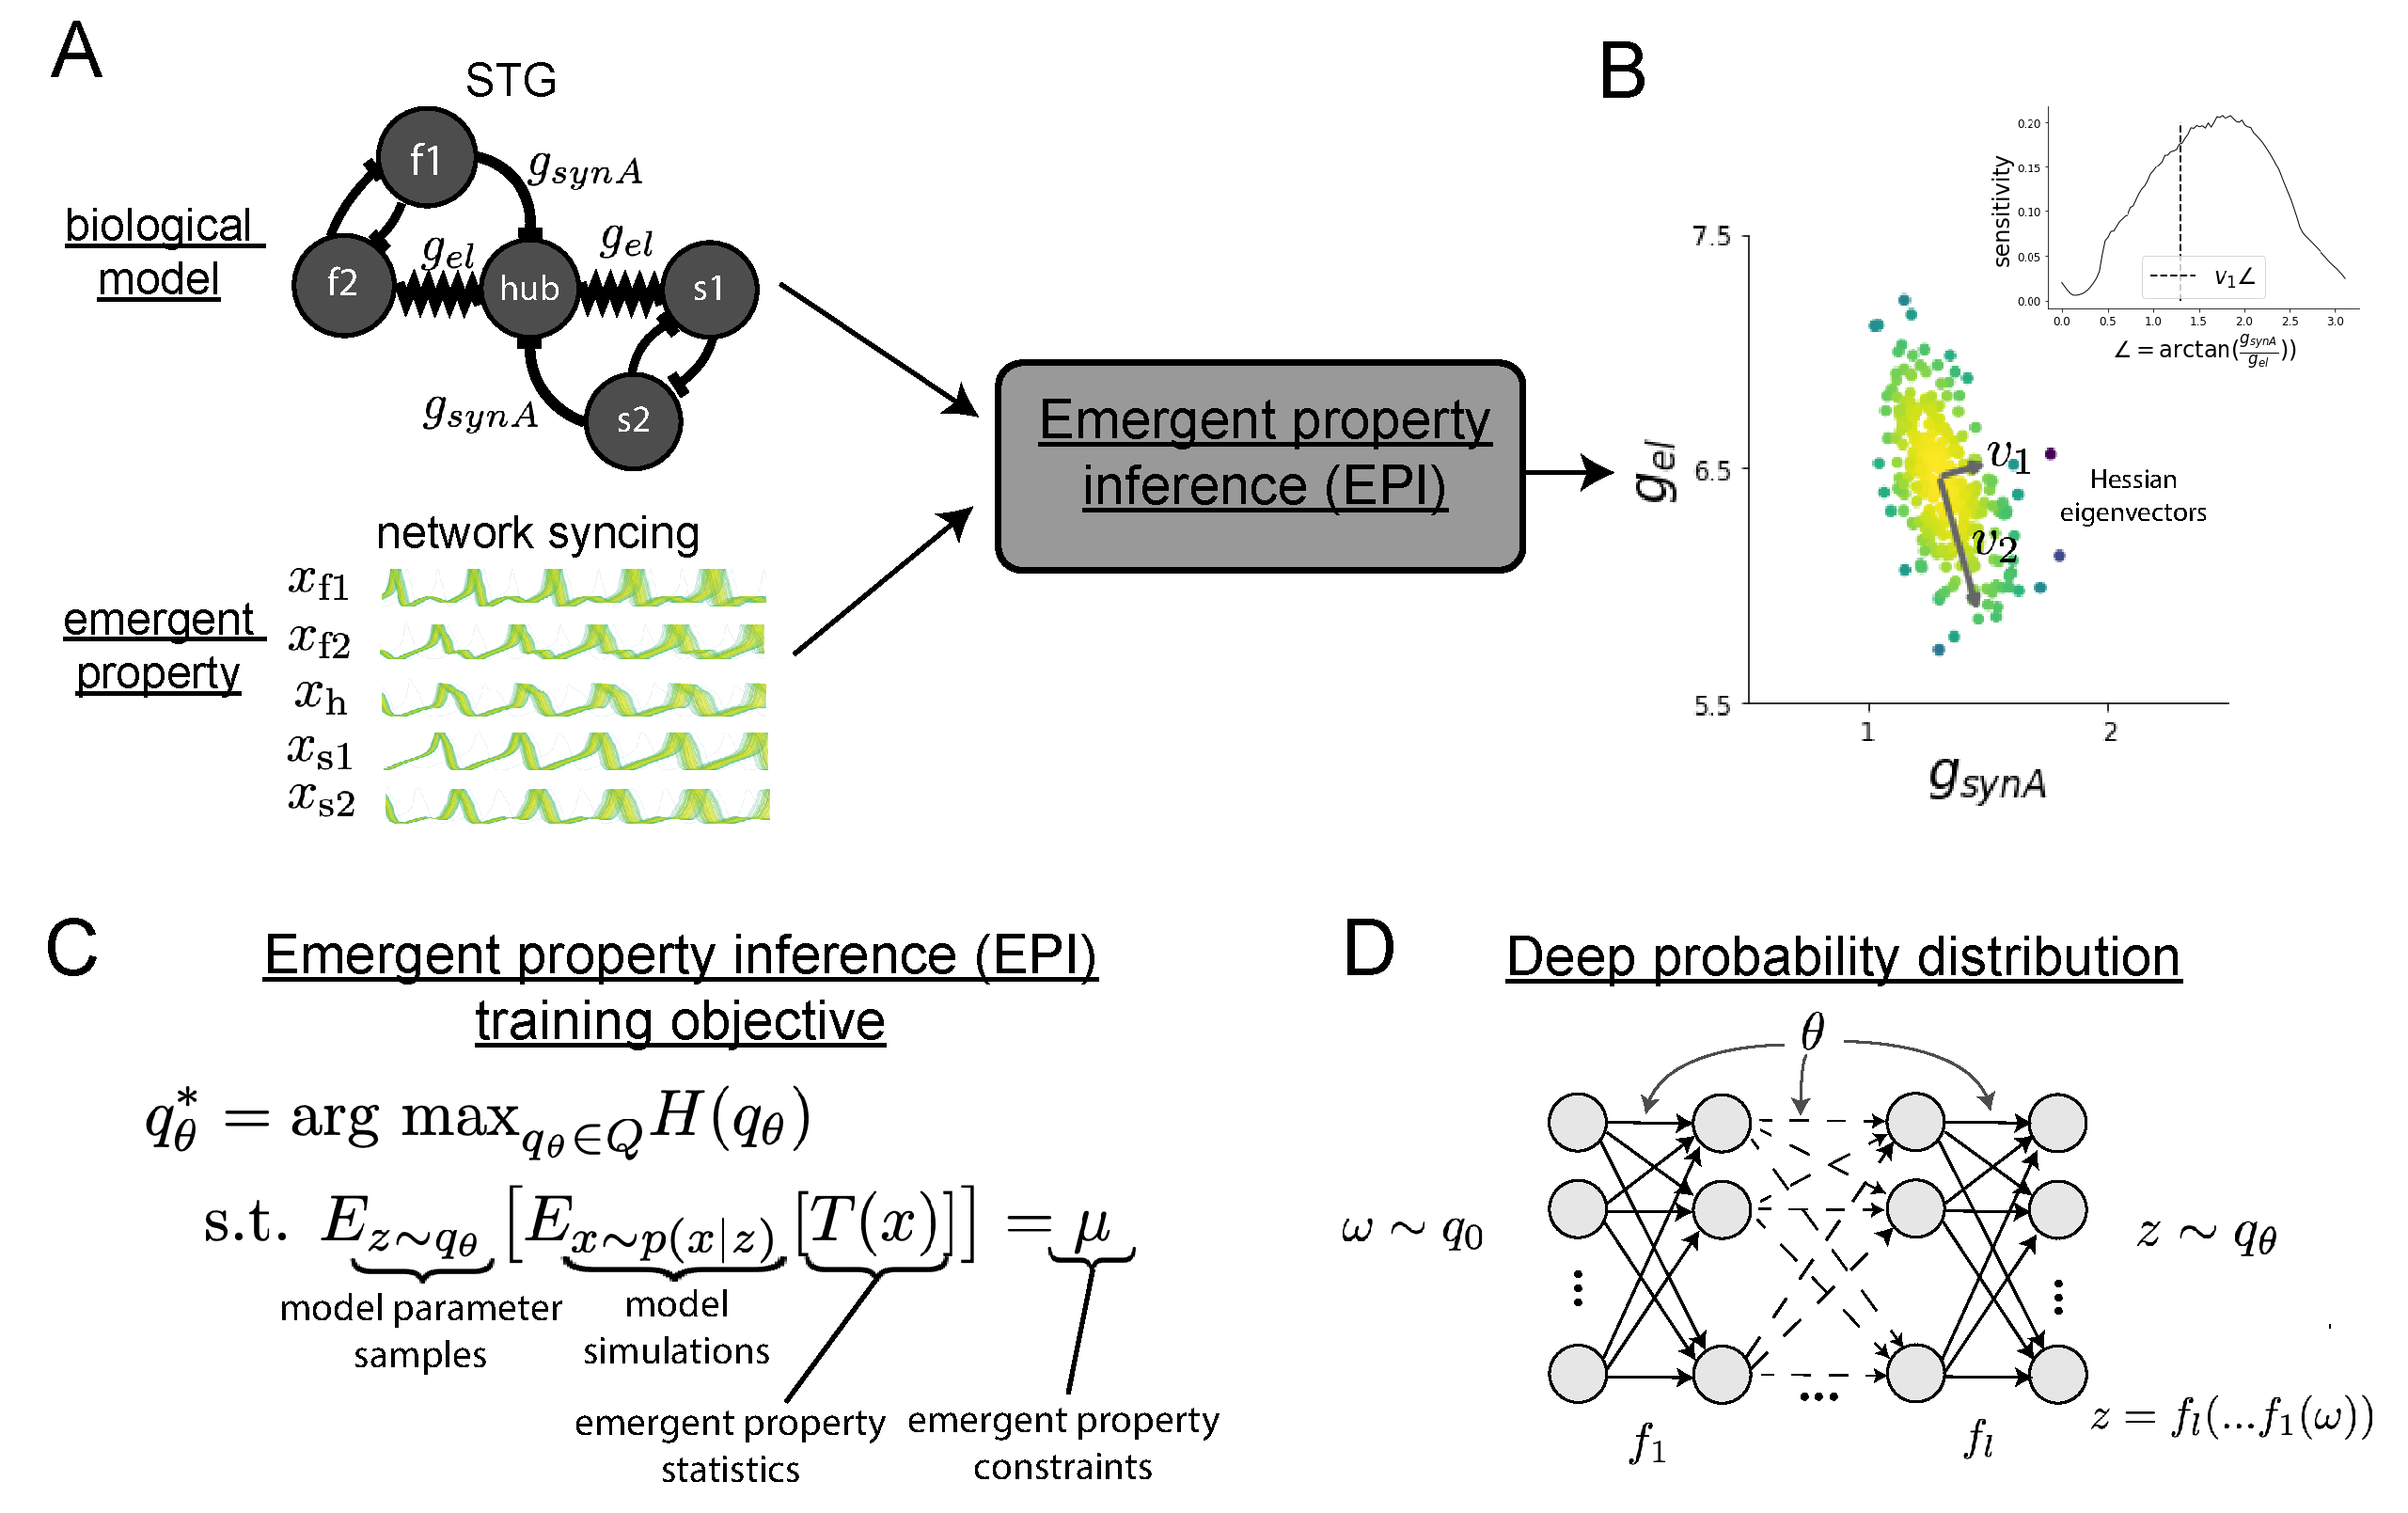
\includegraphics[scale=0.38]{figures/fig1/fig1.pdf}
\end{center}
\caption{Emergent property inference (EPI) in the stomatogastric ganglion.  A. For a choice of model (STG) and emergent property (network syncing), emergent property inference (EPI) learns a posterior distribution of the model parameters  $z = \left[g_{\text{el}}, g_{\text{synA}} \right]^\top$ conditioned on network syncing. B. An EPI distribution of STG model parameters producing network syncing.  The eigenvectors of the Hessian at the mode of the inferred distribution are indicated as $v_1$ and $v_2$.   (Inset) Sensitivity of the system with respect to network syncing along all dimensions of parameter space away from the mode. (see Section \ref{methods_STG}).  C. Deep probability distributions map a latent random variable $\omega \sim q_0$, where $q_0$ is chosen to be simple distribution such as an isotropic Gaussian, through a highly expressive function family $f_\theta(\omega) = f_l(...f_1(\omega))$ parameterized by the neural network weights and biases $\theta \in \Theta$. This mapping induces an implicit probability model $q(g_\theta(\omega)) \in \mathcal{Q}$ D. EPI learns a distribution $q_\theta(z)$ of model parameters that produce an emergent property: the emergent property statistics $T(x)$ are fixed in expectation over parameter distribution samples $z \sim q_\theta(z)$ to particular values $\mu$.  EPI distributions maximize randomness via entropy, although other measures are sensible.  }
\end{figure}


%%%%%%%%%%%%%%%%%%%%%%%%%%%%%%%%%%%
%%%%%%%%%%%%%%%%%%%%%%%%%%%%%%%%%%%


\section{Results}

\subsection{Motivating emergent property inference of theoretical models} \label{results_motivating}

Consideration of the typical workflow of theoretical modeling clarifies the need for emergent property inference.  
First, the theorist designs or chooses an existing model that, it is hypothesized, captures the computation of interest. 
 To ground this process in a well-known example, consider the stomatogastric ganglion (STG) of crustaceans, a small neural circuit which generates multiple rhythmic muscle activation patterns for digestion \cite{marder2002cellular}.
Despite full knowledge of STG connectivity and a precise characterization of its rhythmic pattern generation, biophysical models of the STG have compilcated relationships between circuit parameters and neural activity \cite{prinz2004similar}.
A model of the STG \cite{gutierrez2013multiple} is shown schematically in Figure 1A, and note that the behavior of this model will be critically dependent on its parameterization -- the choices of conductance parameters $z = [g_{\text{el}}, g_{\text{synA}}]$.
Spcecifically, the two fast neurons ($f1$ and $f2$) mutually inhibit one another, and oscillate at a faster frequency than the mutually inhibiting slow neurons ($s1$ and $s2$), and the hub neuron (hub) couples with the fast or slow population or both.  

Second, once the model is selected, the theorist defines the emergent property, the measurable signal of scientific interest.  
To continue our running STG example, one such emergent property is the phenomenon of \emph{network syncing} -- in certain parameter regimes, the frequency of the hub neuron matches that of the fast and slow populations at an intermediate frequency.  This emergent property is shown in Figure 1A at a frequency of 0.55Hz.

Third, qualitative parameter analysis ensues: since precise mathematical analysis is intractable in this model, a brute force sweep of parameters is done \cite{gutierrez2013multiple}.  Subsequently, a qualitative description is formulated to describe of the different parameter configurations that lead to the emergent property.  
In this last step lies the opportunity for a precise quantification of the emergent property as a statistical feature of the model.  Once we have such a methodology, we can infer a probability distribution over parameter configurations that produce this emergent property. 

Before presenting technical details (in the following section), let us understand emergent property inference schematically:  the black box in Figure 1A takes, as input, the model and the specified emergent property, and produces as output the parameter distribution shown in Figure 1B.  
This distribution -- represented for clarity as samples from the distribution -- is then a scientifically meaningful and mathematically tractable object.  
It conveys parameter regions critical to the emergent property, directions in parameter space that will be invariant (or not) to that property, and more.  
In the STG model, this distribution can be specifically queried to determine the prototypical parameter configuration for network syncing (the mode; Figure 1B star), and then how quickly network syncing will decay based on changes away from that mode.  The inset of Figure 1B validates that indeed network syncing behaves as the distribution predicts, when moving away from the mode (Figure 1B star).  
Further validation of EPI is available in the supplementary materials, where we analyze a simpler model for which ground-truth statements can be made (Section \ref{methods_2DLDS}).
%Taken together, bringing careful inference to theoretical models offers deeper insight into the behavior of these models, and the opportunity to make rigorous this last step in the practice of theoretical neuroscience.

\subsection{A deep generative modeling approach to emergent property inference} \label{results_dgm}

Emergent property inference (EPI) systematizes the three-step procedure of the previous section.
First, we consider the model as a coupled set of differential (and potentially stochastic) equations \cite{gutierrez2013multiple}.  In the running STG example, the dynamical state $x = \left[ x_{\text{f1}}, x_{\text{f2}}, x_{\text{hub}}, x_{\text{s1}}, x_{\text{s2}} \right]$ is the membrane potential for each neuron, which evolves according to the biophysical conductance-based equation:
\begin{equation} C_m \frac{dx}{dt} = -h(x; z) = - \left[ h_{leak}(x; z) + h_{Ca}(x; z) + h_K(x; z) + h_{hyp}(x; z) + h_{elec}(x; z) + h_{syn}(x; z)\right] 
\end{equation} 
where $C_m$=1nF, and $h_{\text{leak}}$, $h_{Ca}$, $h_K$, $h_{\text{hyp}}$, $h_{\text{elec}}$, $h_{\text{syn}}$ are the leak, calcium, potassium, hyperpolarization, electrical, and synaptic currents, all of which have their own complicated dependence on $x$ and $z = [g_{\text{el}}, g_{\text{synA}}]$ (see Section \ref{methods_STG}).

Second, we define the emergent property, which as above is network syncing: oscillation of the entire population at an intermediate frequency of our choosing (Figure 1A bottom).
Quantifying this phenomenon is straightforward: we define network syncing to be that each neuron's spiking frequency -- denoted $\omega_{\text{f1}}(x)$, $\omega_{\text{f2}}(x)$, etc. -- is close to an intermediate frequency of 0.55Hz.  
Mathematically, we achieve this via constraints on the mean and variance of $\omega_i(x)$ for each neuron $i \in \{ \text{f1}, \text{f2}, \text{hub}, \text{s1}, \text{s2} \}$, and thus:
\begin{equation}\label{eq:EP}
 E\left[T(x) \right] ~~\triangleq~~ E\begin{bmatrix} \omega_{\text{f1}}(x) \\ \vdots \\ (\omega_{\text{f1}}(x) - 0.55)^2 \\ \vdots \end{bmatrix} ~~=~~  
 \begin{bmatrix} 0.55 \\ \vdots \\ 0.025^2 \\ \vdots \end{bmatrix} ~~\triangleq~~ \mu,
 \end{equation}
  which completes the quantification of the emergent property.

Third, we perform emergent property inference: we find a distribution over parameter configurations $z$, and insist that samples from this distribution produce the emergent property; in other words, they obey the constraints introduced in Equation \ref{eq:EP}.  
This distribution will be chosen from a family of probability distributions $\mathcal{Q} = \left\{ q_\theta(z) : \theta \in \Theta \right\}$, defined by a deep generative distribution
of the normalizing flow class \cite{rezende2015variational, dinh2016density, papamakarios2017masked} -- neural networks which transform a simple distribution into a suitably complicated distribution (as is needed here).  
This deep distribution is represented in Figure 1C (and see Methods for more detail).  
Then, mathematically, we must solve the following optimization program: 
 \begin{equation} \label{eq:EPI}
\begin{split}
&\argmax_{q_\theta \in \mathcal{Q}} H(q_\theta(z)) \\
 &\text{  s.t.  } E_{z \sim q_\theta}\left[ E_{x\sim p(x \mid z)}\left[T(x)\right] \right] = \mu, \\
\end{split}
\end{equation}
where $T(x), \mu$ are defined as in Equation \ref{eq:EP}, and $p(x|z)$ is the intractable distribution of data from the model ($x$), given that model's parameters $z$ (we access samples from this distribution by running the model forward).   The purpose of each element in this program is detailed in Figure 1D.
Finally, we recognize that many distributions in $\mathcal{Q}$ will respect the emergent property constraints, so we require a normative principle to select amongst them.  
This principle is captured in Equation \ref{eq:EPI} by the primal objective $H$.  
Here we chose Shannon entropy as a means to find parameter distributions with minimal assumptions beyond some chosen structure \cite{jaynes1957information, elsayed2017structure, loaiza2017maximum, savin2017maximum}, but we emphasize that the EPI method is unaffected by this choice (but the results of course will depend on the primal objective chosen).  
%Stating such a problem is easy enough; finding a tractable and suitably flexible family of probability distributions ($\mathcal{Q}$) is hard.  
%With normalizing flows, we leverage the tractable calculation of log sample probability $\log q_\theta(z)$ to optimize entropy \cite{loaiza2017maximum}.
%One can interpret the resulting probabilities as increasing with closeness in emergent property statistics to the emergent property values (see Section \ref{methods_2DLDS}).

EPI optimizes the weights and biases $\theta$ of the deep neural network (which induces the probability distribution) by iteratively solving Equation \ref{eq:EPI}. 
The optimization is complete when the sampled models with parameters $z \sim q_\theta$ produce activity consistent with the specified emergent property.  
Such convergence is evaluated with a hypothesis test that the mean of each emergent property statistic is not different than its emergent property value (see Section \ref{methods_AL_opt}). 
Equipped with this method, we now prove out the value of EPI by using it to investigate three prominent models in neuroscience, using EPI to produce new insights about these models.


%%%%%%%%%%%%%%%%%%%%%%%%%%%%
\subsection{Comprehensive input-responsivity in a nonlinear sensory system} \label{results_V1}

\begin{figure}
\begin{center}
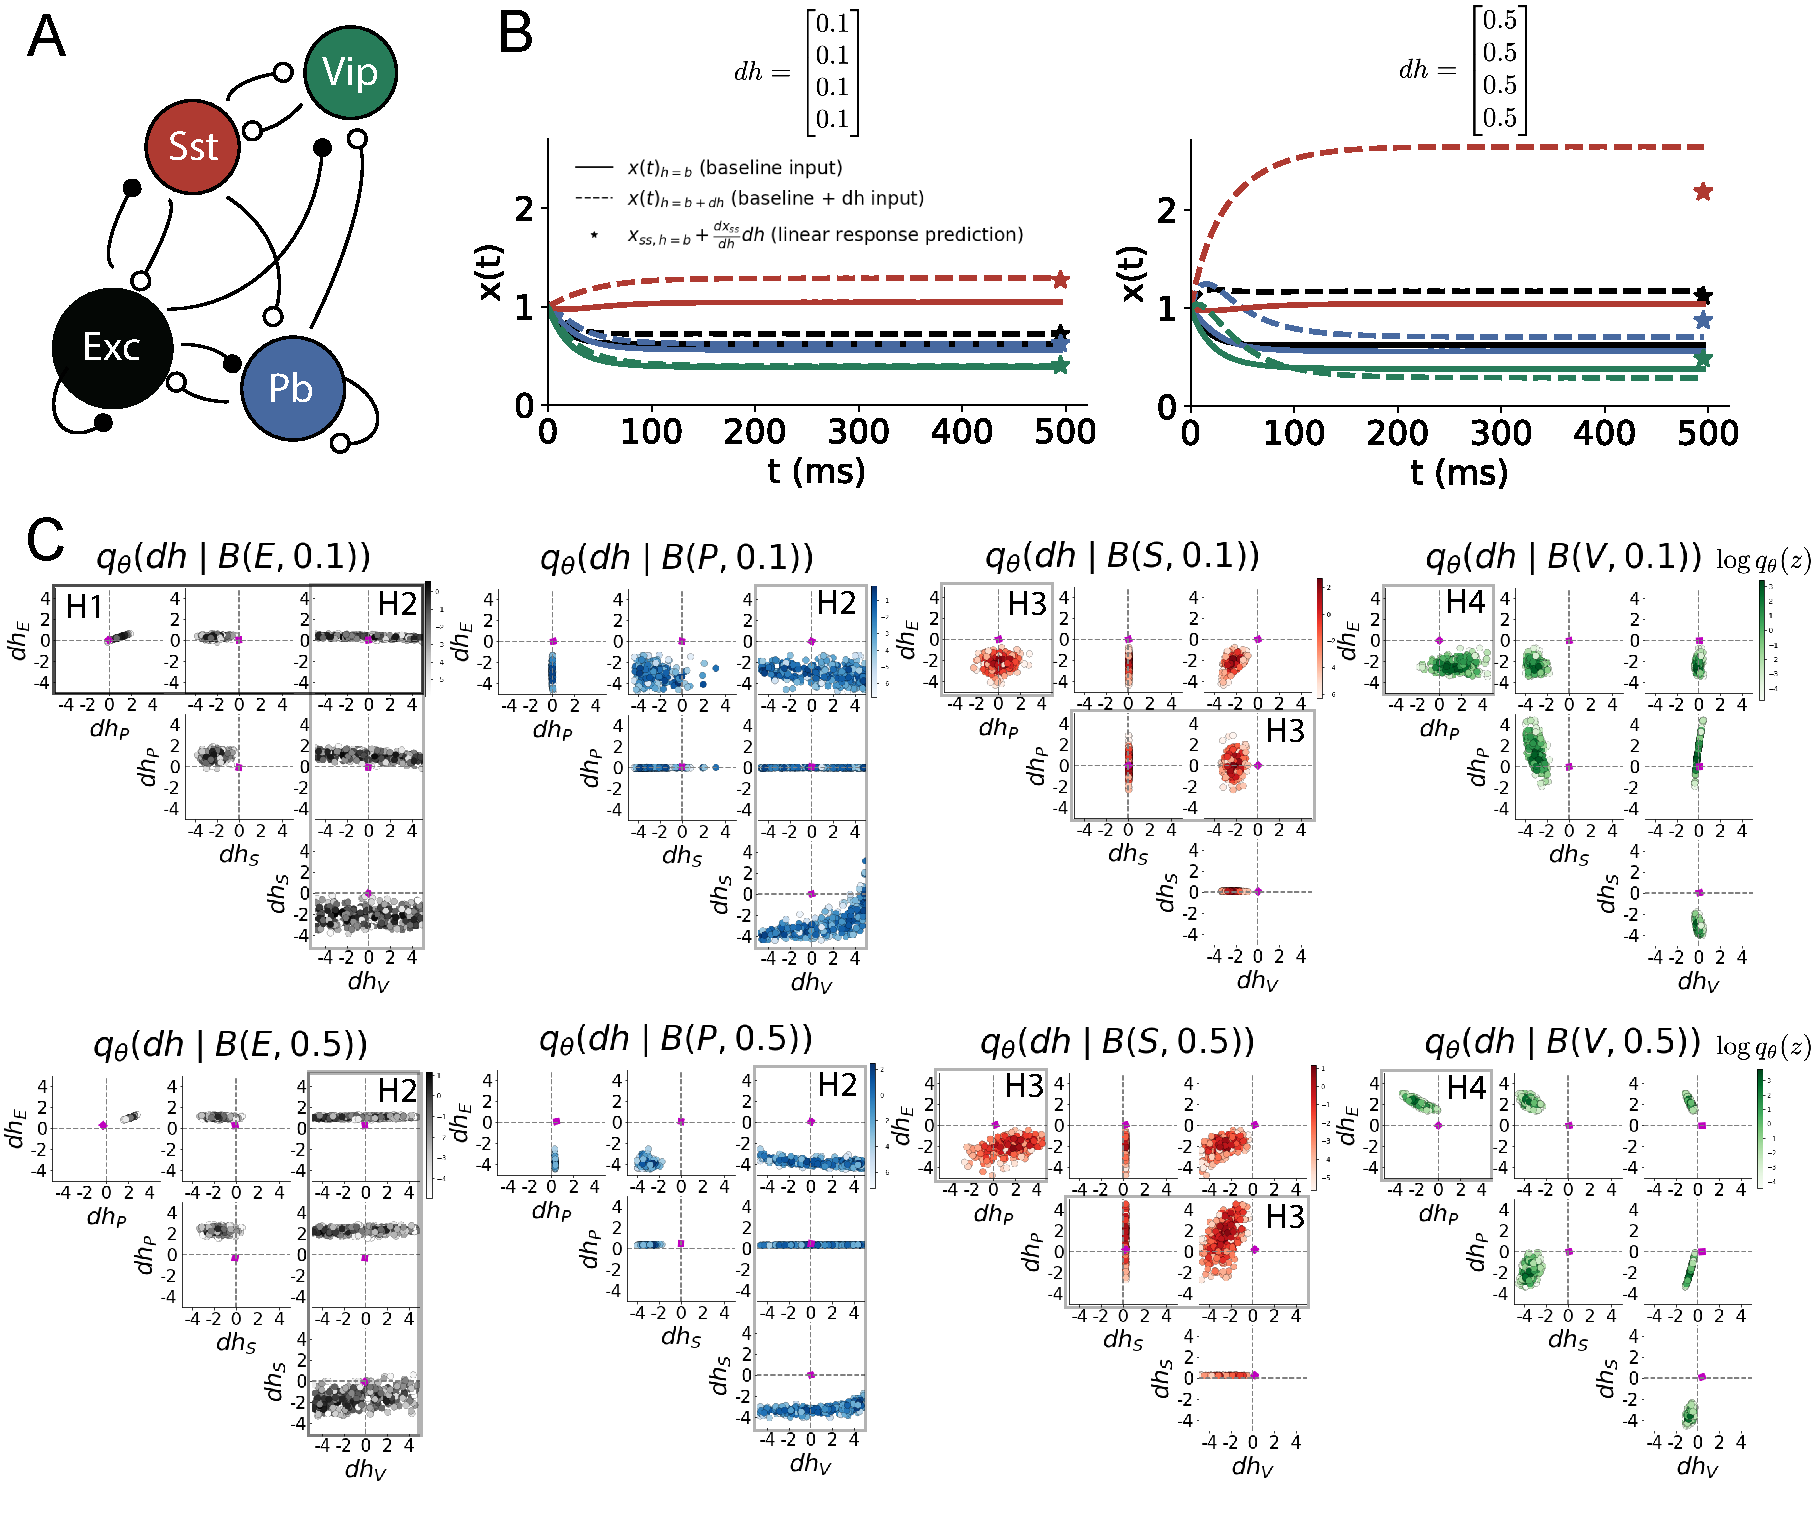
\includegraphics[scale=0.55]{figures/fig2/fig2.pdf}
\end{center}
\caption{Hypothesis generation through EPI in a V1 model.  A. Four-population model of primary visual cortex with excitatory (black), parvalbumin (blue), somatostatin (red), and vip (green) neurons.   Some neuron-types largely do not form synaptic projections to others  (excitatory and inhibitory projections filled and unfilled, respectively).  B. Linear response predictions become inaccurate with greater input strength.  V1 model simulations for input (solid) $h=b$ and (dashed) $h = b + dh$ with $b = \left[1, 1, 1, 1\right]\top$ and (left) $dh = \left[0.1, 0.1, 0.1, 0.1\right]\top$ (right) $dh = \left[0.5, 0.5, 0.5, 0.5\right]\top$.  Stars indicate the linear response prediction.  C. EPI distributions on differential input $dh$ conditioned on differential response $\mathcal{B}(\alpha, y)$. Supporting evidence for the four generated hypotheses are indicated by gray boxes with labels H1, H2, H3, and H4. The linear prediction from two standard deviations away from $y$ (from negative to positive) is overlaid in magenta (very small, near origin). }
\end{figure}

In studies of primary visual cortex (V1), theoretical models with excitatory (E) and inhibitory (I) populations have reproduced a host of experimentally documented phenomena. 
  In particular regimes of excitation and inhibition, these E/I models exhibit the paradoxical effect \cite{tsodyks1997paradoxical}, selective amplification \cite{murphy2009balanced}, surround suppression \cite{ozeki2009inhibitory}, and  sensory integrative properties \cite{rubin2015stabilized}.  
 Extending this model using experimental evidence of three genetically-defined classes of inhibitory neurons \cite{markram2004interneurons, rudy2011three}, recent work \cite{litwin2016inhibitory} has investigated a four-population model --  excitatory (E), parvalbumin (P), somatostatin (S), and vasointestinal peptide (V) neurons -- as shown in Fig. 2A.
 The dynamical state of this model is the firing rate of each neuron-type population $x = \left[x_E, x_P , x_S, x_V \right]^\top$, which evolves according to rectified ($\left[ \right]_+$) and exponentiated dynamics:
%
\begin{equation}
\tau \frac{dx}{dt} = -x + [W x+ h]_+^n
\end{equation}
%
with effective connectivity weights $W$ and input $h$.  In our analysis, we set the time constant $\tau = 20$ms and dynamics coefficient $n = 2$.  
Also, as is fairly standard, we obtain an informative estimate of the effective connectivities between these neuron-types $W$ in mice by multiplying their probability of connection with their average synaptic strength \cite{allen2018layer, billeh2019systematic} (see Section \ref{methods_V1}).
Given these fixed choices of $W$, $n$, and $\tau$, we studied the system's response to input
\begin{equation}
h = b + dh,
\end{equation} 
where the input $h$ is comprised of a baseline input $b = \left[ b_E, b_P , b_S , b_V \right]^\top$ and a differential input $dh = \left[ dh_E , dh_P , dh_S , dh_V\right]^\top$ to each neuron-type population.  Throughout subsequent analyses, the baseline input is $b = \left[ 1 ,1,1,1\right]^\top$. 

Having established our model, we now define the emergent property. We begin with the linearized response of the system to input $\frac{dx_{ss}}{dh}$ at the steady state $x_{ss}$, i.e. a fixed point. 
While this linearization accurately predicts differential responses $dx_{ss} = \left[ dx_{E,ss} , dx_{P,ss} , dx_{S,ss} ,dx_{V,ss} \right]$  for small differential inputs to each population $dh = \left[ 0.1 , 0.1 , 0.1 , 0.1 \right]$ (Fig. 2B, left), linearization is a poor predictor in this nonlinear model more generally (Fig. 3B, right). 
Currently available approaches to deriving the steady state response of this system are limited.

To get a more comprehensive picture of the input-responsivity of each neuron-type, we used EPI to learn a distribution of the differential inputs to each population $dh$ that produce an increase of $y \in \{0.1, 0.5\}$ in the rate of each neuron-type population $\alpha \in \{E, P, S, V \}$.  
We want to know the differential inputs $dh$ that result in a differential steady state $dx_{\alpha,ss}$ (the change in $x_{\alpha,ss}$ when receiving input $h=b + dh$ with respect to the baseine $h = b$) of value $y$ with some small, arbitrarily chosen amount of variance  $0.01^2$.   
These statements amount to the emergent property 
\begin{equation}
\mathcal{B}(\alpha, y) ~~\triangleq~~ 
E \begin{bmatrix} dx_{\alpha,ss} \\ (dx_{\alpha,ss} - y)^2 \end{bmatrix} ~~=~~ \begin{bmatrix} y \\ 0.01^2 \end{bmatrix}
\end{equation}
We continue to use $\mathcal{B}(\cdot)$ throughout the rest of the study as short hand for emergent property, which represents a different signature of computation in each application. In Each column of Figure 2C visualizes the inferred distribution of $dh$ corresponding to a excitatory (red), parvalbumin (blue), somatostatin (red) and vip (green) neuron-type increase, while each row corresponds to amounts of increase 0.1 and 0.5.  These distributions conditioned on such emergent properties are now available through EPI. For each pair of parameters we show the two-dimensional marginal distribution of samples colored by $\log q_\theta(dh \mid \mathcal{B}(\alpha, y))$.  The inferred distributions immediately suggest four hypotheses: \\

{\addtolength{\leftskip}{10 mm}
H1: as is intuitive, each neuron-type's firing rate should be sensitive to that neuron-type's direct input (e.g. Fig. 2C H1 indicates low variance in $dh_E$ when $\alpha=E$. Same observation in all inferred distributions); \\
H2: the E- and P-populations should be largely unaffected by $dh_V$ (Fig. 2C H2 indicates high variance in $dh_V$ when $\alpha \in \{E, P \}$); \\
H3: the S-population should be largely unaffected by $dh_P$  (Fig. 2C H3 indicate high variance in $dh_P$ when $\alpha =S$); \\
H4: there should be a nonmonotonic response of $dx_{V,ss}$ with $dh_{E}$ (Fig. 2C H4 indicates that negative $dh_E$ should result in small $dx_{V,ss}$, but positive $dh_E$ should elicit a larger $dx_{V,ss}$);

}

\begin{figure}
\floatbox[{\capbeside\thisfloatsetup{capbesideposition={right,top},capbesidewidth=4cm}}]{figure}[\FBwidth]
{\caption{Confirming EPI generated hypotheses in V1. A. Differential responses by the E-population to changes in individual input $\Delta h_\alpha u_\alpha$ away from the mode of the EPI distribution $dh^*$. B-D Same plots for the P-, S-, and V-populations.  Labels H1, H2, H3, and H4 indicate which curves confirm which hypotheses.}}
{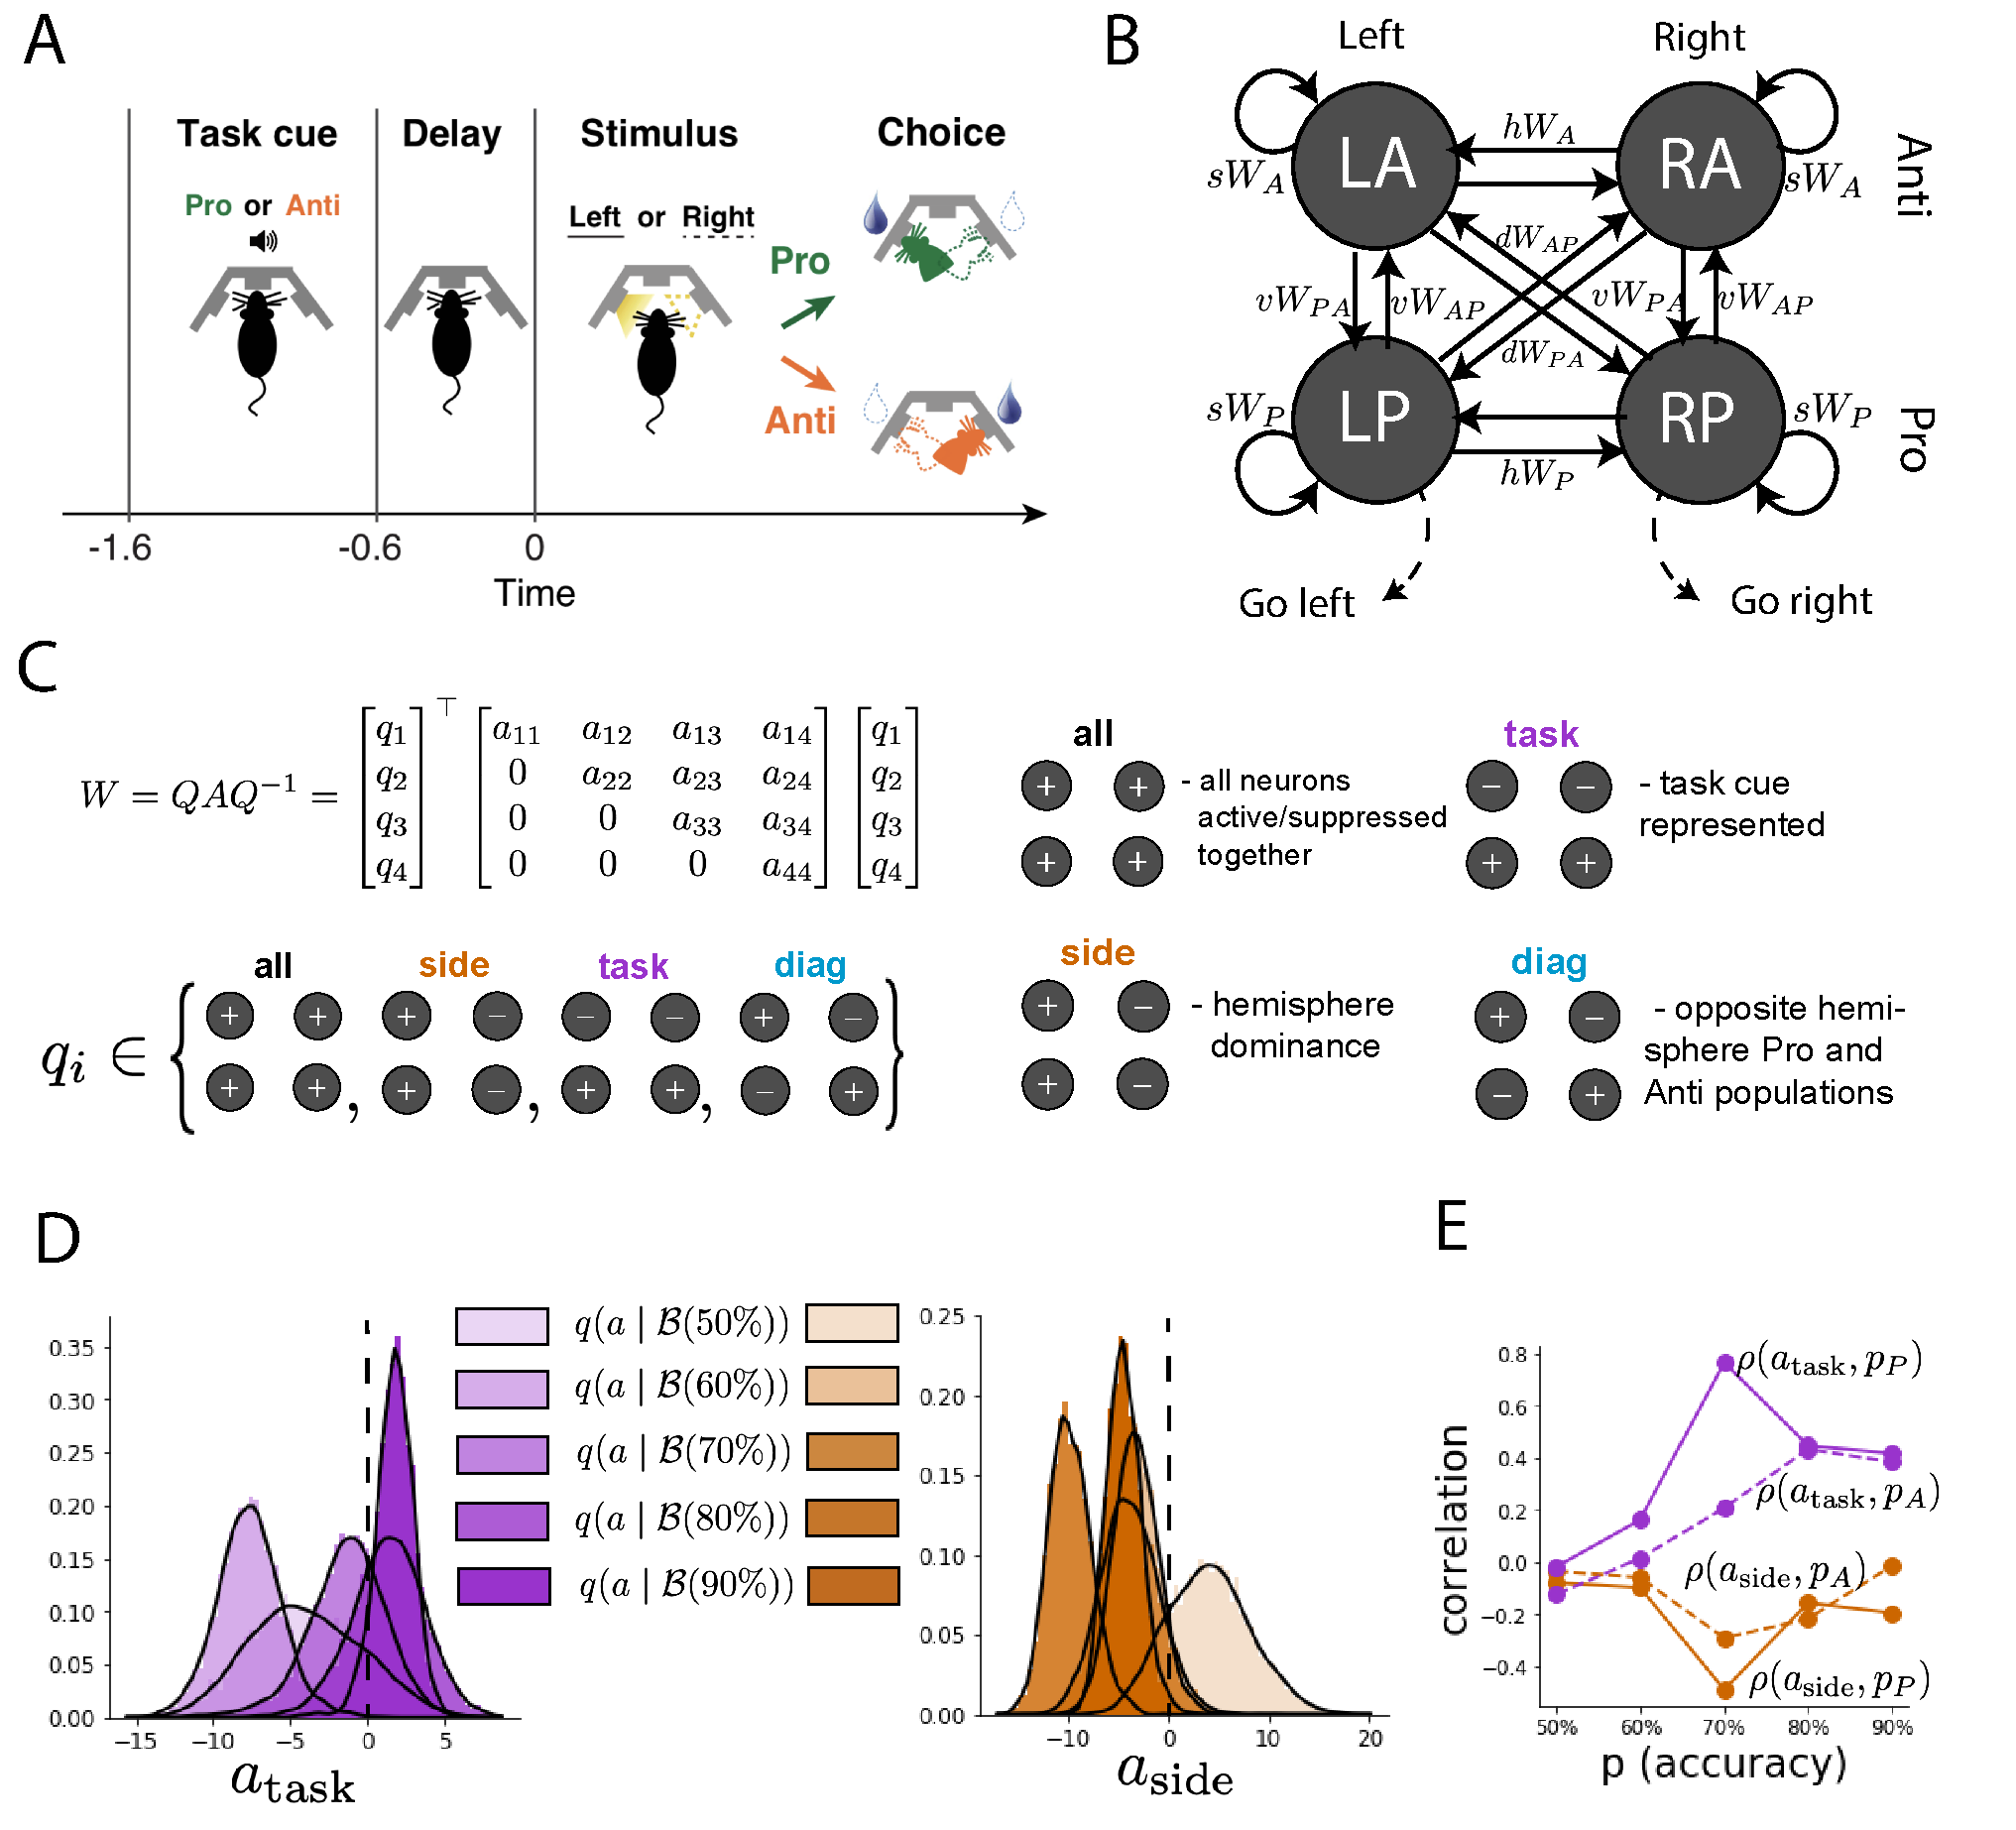
\includegraphics[scale=0.6]{figures/fig3/fig3.pdf}}
\end{figure}

We evaluate these hypotheses by taking steps in individual neuron-type input $\Delta h_\alpha$ away from the modes of the inferred distributions at $y=0.1$.
\begin{equation}
dh^* = z^* = \argmax_{z} \log q_\theta(z \mid \mathcal{B}(\alpha, 0.1))
\end{equation}
Now, $dx_{\alpha,ss}$ is the steady state response to the system with input $h = b + dh^* + \Delta h_\alpha u_\alpha$ where $u_\alpha$ is a unit vector in the dimension of $\alpha$. The EPI-generated  hypotheses are confirmed. 
\begin{itemize}
\item the neuron-type responses are sensitive to their direct inputs (Fig. 3A black, 3B blue, 3C red, 3D green);
\item  the E- and P-populations are not affected by $dh_V$ (Fig. 3A green, 3B green);
\item the S-population is not affected by $dh_P$ (Fig. 3C blue);
\item the V-population exhibits a nonmonotonic response to $dh_E$ (Fig. 3D black), and is in fact the on population to do so (Fig. 3A-C black).
\end{itemize}

These hypotheses were in stark contrast to what was available to us via traditional analytical linear prediction (Fig. 2C, magenta).
To this point, we have shown the utility of EPI on relatively low-level emergent properties like network syncing and differential neuron-type population responses.  
In the remainder of the study, we focus on using EPI to understand models of more abstract cognitive function.

%%%%%%%%%%%%%%%%%%%%%%%%
\subsection{Identifying neural mechanisms of behavioral learning.} \label{results_SC}
Identifying measurable biological changes that result in improved behavior is important for neuroscience, since they may indicate how the learning brain adapts.
In a rapid task switching experiment \cite{duan2015requirement}, rats were explictly cued on each trial to either orient towards a visual stimulus in the Pro (P) task or orient away from a visual stimulus in the Anti (A) task (Fig. 3a). Neural recordings in the midbrain supeior colliculus (SC) exhibited two population of neurons that simultaneously represented both task context (Pro or Anti) and motor response (contralateral or ipsilateral to the recoreded side): the Pro/Contra and Anti/Ipsi neurons \cite{duan2018collicular}.
Duan et al. proposed a model of SC that, like the V1 model analyzed in the previous section, is a four-population dynamical system.  
Here, the neuron-type populations are functionally-defined as the Pro- and Anti-populations in each hemisphere (left (L) and right (R)).  
The Pro- or Anti-populations receive an input determined by the cue, and then the left and right populations receive an input based on the side of the light stimulus. 
Activities were bounded between $0$ and $1$, so that a high output of the Pro population in a given hemisphere corresponds to the contralateral response.   
An additional stipulation is that when one Pro population responds with a high-output, the opposite Pro population must respond with a low output.
Finally, this circuit operates in the presence of Gaussian noise resulting in trial-to-trial variability (see Section \ref{methods_SC}).
The connectivity matrix is parameterized by the geometry of the population arrangement (Fig. 3B).  

Here, we used EPI to learn distributions of the SC weight matrix parameters $z = W$ conditioned on of various levels of rapid task switching accuracy $\mathcal{B}(p)$ for $p \in \{50\%, 60\%, 70\%, 80\%, 90\%\}$ (see Section \ref{methods_SC}).  Following the approach in Duan et al., we decomposed the connectivity matrix $W = QAQ^{-1}$ in such a way (the Schur decomposition) that the basis vectors $q_i$ are the same for all $W$ (Fig. 3C). These basis vectors have intuitive roles in processing for this task, and are accordingly named the \textit{all} mode - all neurons co-fluctuate, \textit{side} mode - one side dominates the other, \textit{task} mode - the Pro or Anti populations dominate the other, and \textit{diag} mode - Pro- and Anti-populations of opposite hemispheres dominate the opposite pair. The corresponding eigenvalues (e.g. $a_{\text{task}}$, which change according to $W$) indicate the degree to which activity along that mode is increased or decreased by $W$.  

\begin{figure}
\begin{center}
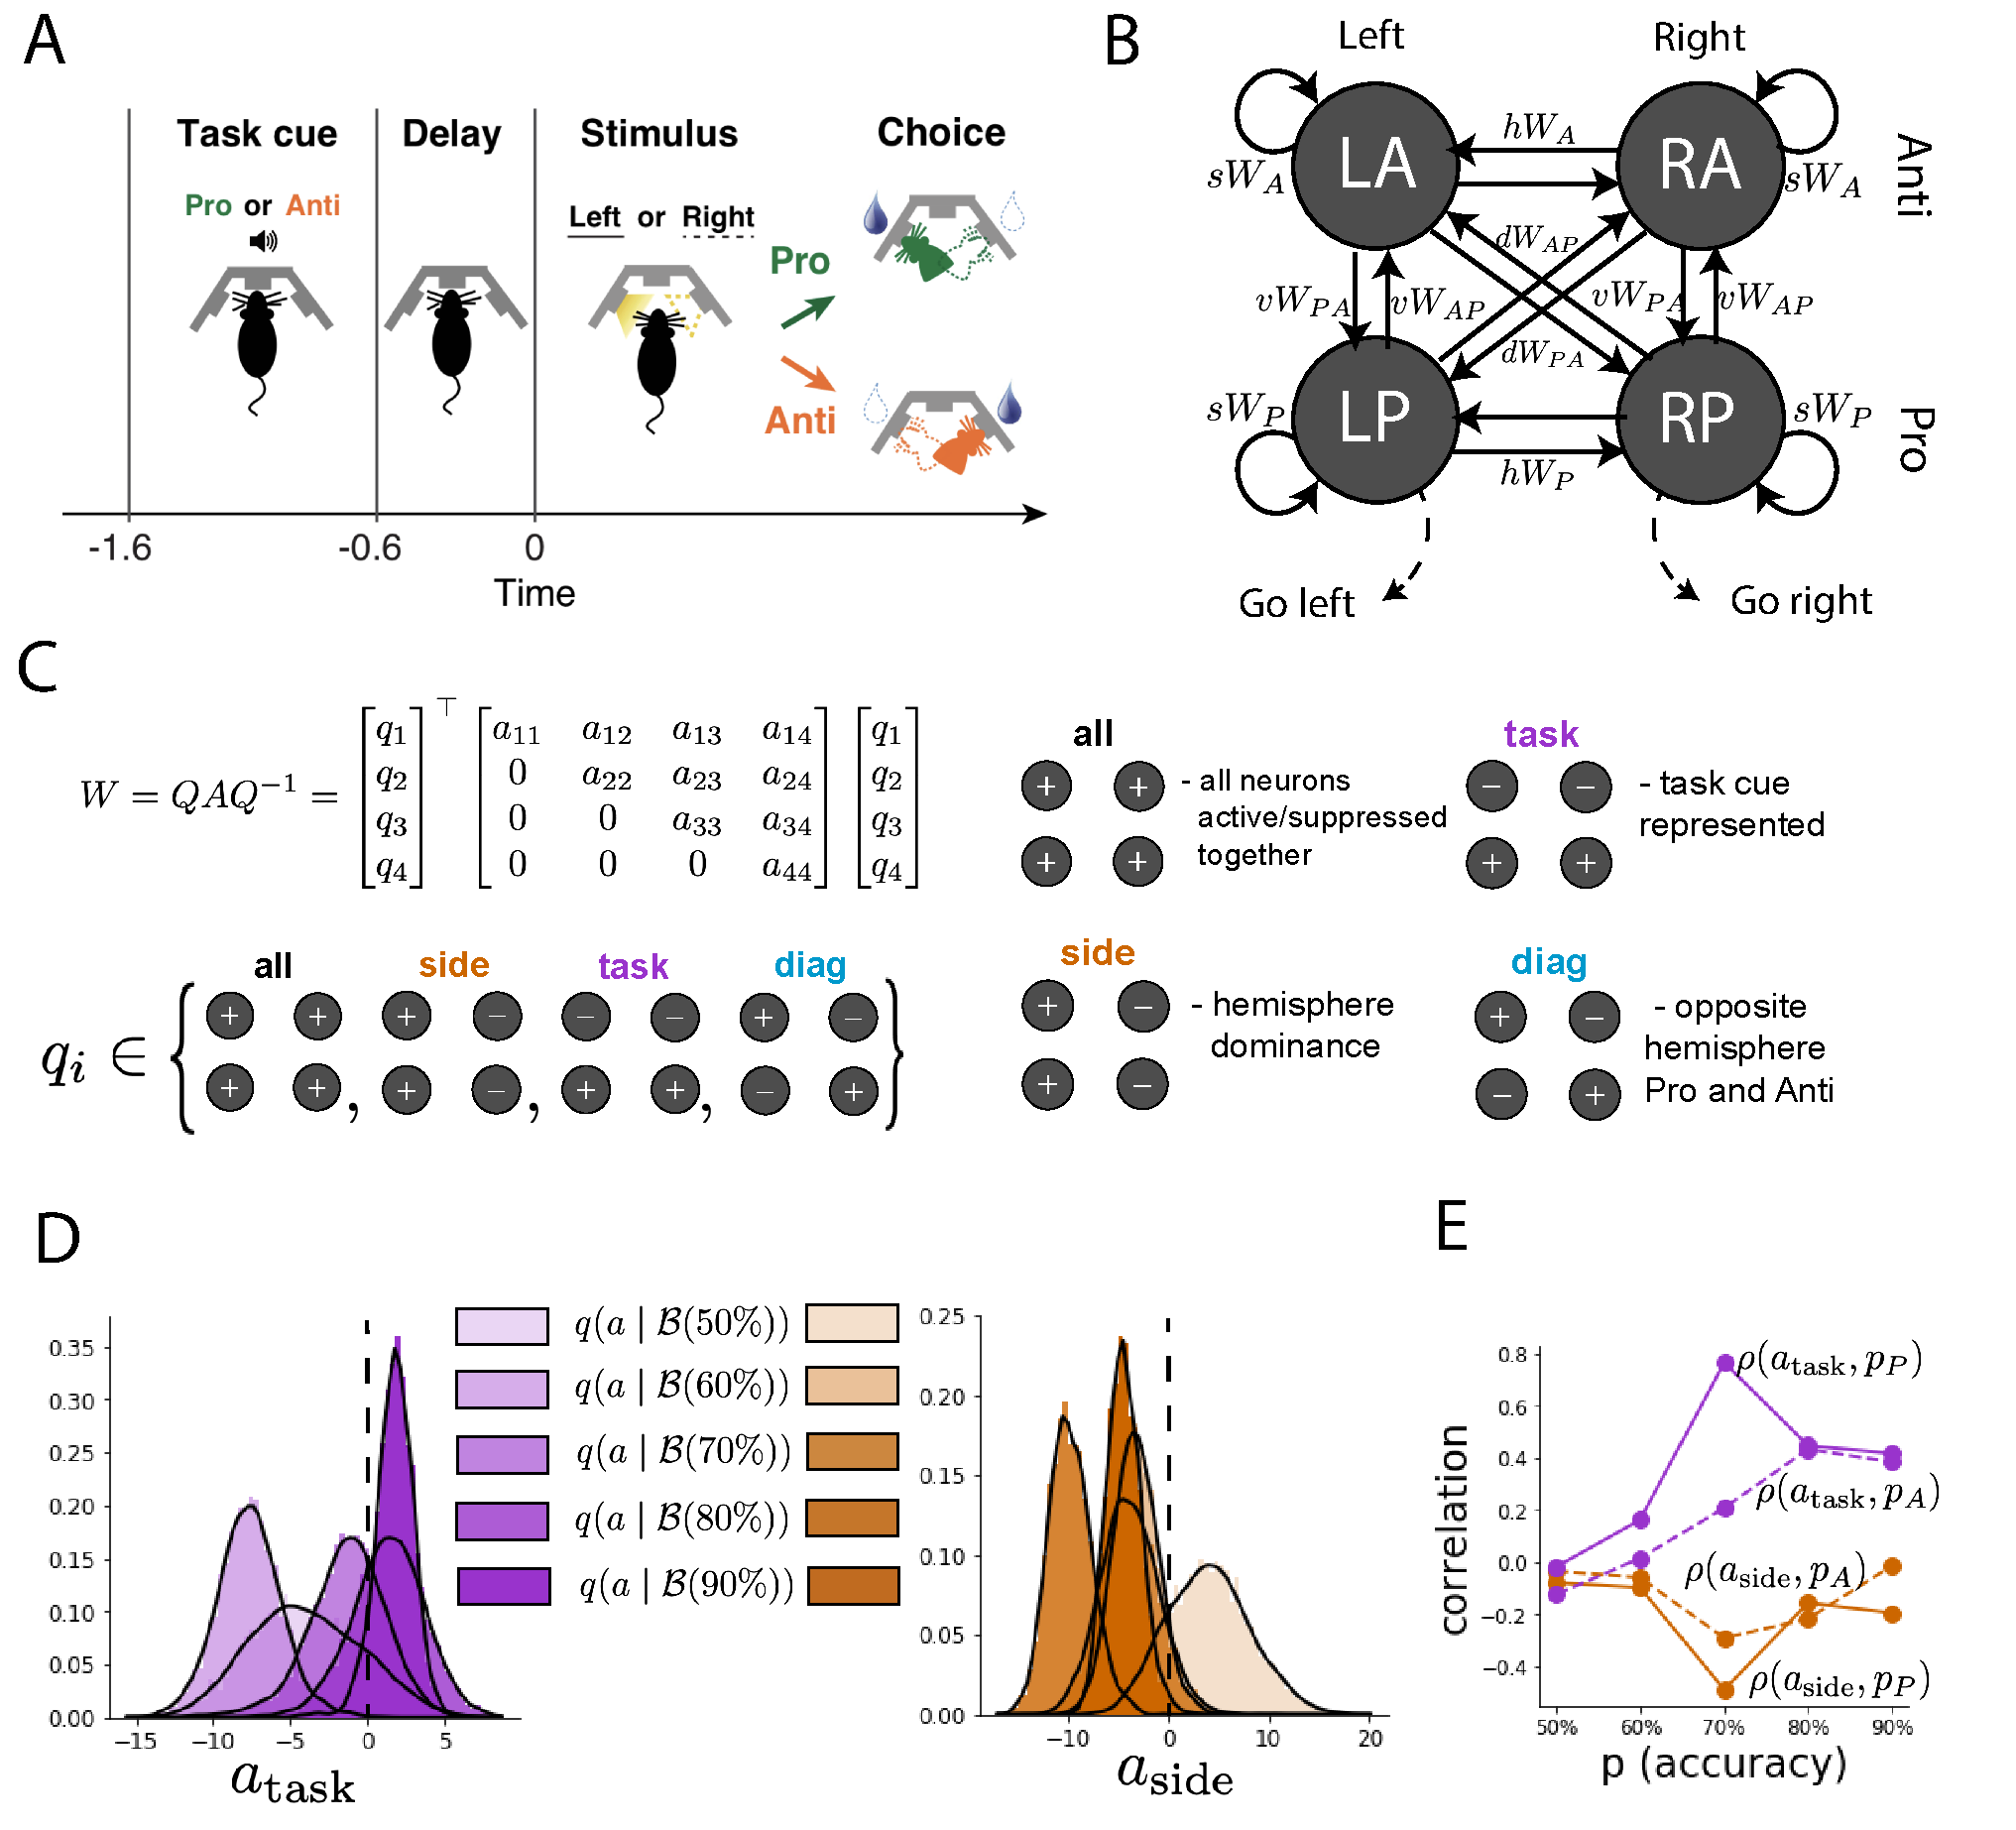
\includegraphics[scale=0.5]{figures/fig4/fig4.pdf}
\end{center}
\caption{EPI reveals changes in SC \cite{duan2018collicular} connectivity that control task accuracy.  A. Rapid task switching behavioral paradigm (see text). B. Model of superior colliculus (SC). Neurons: LP - left pro, RP - right pro, LA - left anti, RA - right anti.  Parameters: sW - self, hW - horizontal, vW -vertical, dW - diagonal weights. C. The Schur decomposition of the weight matrix $W = QAQ^{-1}$ is a unique decomposition with orthogonal $Q$ and upper triangular $A$. Schur modes: $q_{\text{all}}$, $q_{\text{task}}$, $q_{\text{side}}$, and $q_{\text{diag}}$.  D. The marginal EPI distributions of the Schur eigenvalues at each level of task accuracy. E. The correlation of Schur eigenvalue with task performance in each learned EPI distribution.}
\end{figure}

EPI demonstrates that, for greater task accuracies, the task mode eigenvalue increases, indicating the importance of $W$ to the task representation (Fig. 4D, purple).  Stepping from random chance (50\%) networks to marginally task-performing (60\%) networks, there is a marked decrease of the side mode eigenvalues (Fig. 3D, orange).  Such side mode suppression remains in the models achieving greater accuracy, revealing its importance towards task performance.   There were no interesting trends with learning in the all or diag mode (hence not shown in Fig. 3). Importantly, we can conclude from our methodology that side mode suppression in $W$ allows rapid task switching, and that greater task-mode representations in $W$ increase accuracy.  These hypotheses are confirmed by forward simulation of the SC model (Fig. 3E).  Thus, EPI produces novel, experimentally testable predictions: effective connectivity between these populations changes throughout learning, in a way that increases its task mode and decreases its side mode eigenvalues.

%%%%%%%%%%%%%%%%%%%%%%%%
\subsection{Characterizing biases in RNNs solving a posterior conditioning task} \label{results_RNN}
So far, each model we have studied was designed from fundamental biophysical principles, genetically- or functionally-defined neuron types.  
At a more abstract level of modeling, recurrent neural networks (RNNs) are high-dimensional dynamical models of computation becoming increasingly popular in neuroscience research \cite{barak2017recurrent}. 
In theoretical neuroscience, RNNs dynamics usually follow the equation
\begin{equation}
\frac{dx}{dt} = -x(t) + W \phi(x(t)) + I(t),
\end{equation}
where $x(t)$ is the network activity, $W$ is the network connectivity, $\phi(\cdot) = \tanh(\cdot)$, and $I(t)$ is the input to the system.
Such RNNs are trained to do a task from a systems neuroscience experiment, and then the unit activations of the trained RNN are compared to recorded neural activity.
Such highly parameterized models are challenging to characterize, let alone probabilistically infer. 
Predominantly, our understanding of RNN function comes from the identification of fixed points and their local linearized dynamics \cite{sussillo2013opening}, yet these analyses do not afford a direct link between macroscopic connectivity parameters and dynamics.
Alternatively, we use EPI to characterize the parameteric sources of solution bias in an RNN solving a toy mathematical problem.

Here, the task we consider is Gaussian posterior conditioning: calculate the parameters of a Gaussian posterior distribution on the mean of a Gaussian likelihood $\mu_y$, given a single observation of $y \sim \mathcal{N}(\mu_y,\sigma^2_y = 1)$ and a prior $p(\mu_y) = \mathcal{N}(\mu_0=4, \sigma_0^2=1)$ (Fig. 5A).  Conjugacy in the Gaussian likelihood and prior result in ground truth calculation for the Gaussian posterior mean 
\begin{equation}
\mu_{\text{post}} = \frac{\frac{\mu_0}{\sigma_0^2} + \frac{y}{\sigma_y^2}}{\frac{1}{\sigma_0^2} + \frac{1}{\sigma_y^2}}
\end{equation}
 and posterior variance 
\begin{equation}
 \sigma^2_{\text{post}} = \frac{1}{\frac{1}{\sigma_0^2} + \frac{1}{\sigma_y^2}}
\end{equation}
First, we predicate that the RNN should produce activity along a readout vector $w$ corresponding to its estimation of the posterior mean $\mu_{\text{post}}$. Second, we ask that the RNN produce a degree of chaotic variability matching the posterior variance $\sigma^2_{\text{post}}$.  This problem setup is inspired by dynamical systems modeling of approximate inference in the brain \cite{echeveste2019cortical}.  Although, we avoid using the term ``approximate inference" to describe this task, since we are demonstrating the utility of EPI, which is a different form of approximate inference (see Section \ref{methods_VI}).

Drawing conclusions about the role tens of thousands of weight matrix parameters in producing a readout projection and chaotic variance is a daunting challenge.  However, we can leverage recent theoretical work establishing a link between macroscopic parameterizations of RNN connectivity and the emerging dynamics \cite{mastrogiuseppe2018linking}.  Specifically, we consider an $N$-neuron, rank-1 RNN with connectivity
\begin{equation}
W = g\chi + \frac{1}{N}mn^\top,
\end{equation}
where $\chi_{ij} \sim \mathcal{N}(0, \frac{1}{N})$, $g$ is the random strength, and the entries of $m$ and $n$ are drawn from Gaussian distributions $m_i \sim \mathcal{N}(M_m, 1)$ and $n_i \sim \mathcal{N}(M_n, 1)$.  
This theory allows us to calculate the RNN response along a readout vector 
\begin{equation}
\kappa_w =  \frac{1}{N} \sum_{j=1}^N w_j \phi(x_j)
\end{equation}
to a constant input $I(t) = y w + (n-M_n)$.  Additionally, the amount of chaotic variance $\Delta_T$ can be expressed through consistency equations of dynamic mean field parameters, the solver of which we take gradients through (see Section \ref{methods_LRRNN}).
This theory allows us to mathematically formalize the execution of this task into an emergent property, where the emergent property statistics of the RNN activity are $k_w$ and $\Delta_T$ and the emergent property values are the ground truth $\mu_{\text{post}}$ and $\sigma^2_{\text{post}}$:
\begin{equation}
E \begin{bmatrix} \kappa_w \\ \Delta_T \\ (\kappa_w-\mu_{\text{post}})^2 \\ (\Delta_T^2-\sigma^2_{\text{post}}) \end{bmatrix} ~~=~~ \begin{bmatrix} \mu_{\text{post}} \\ \sigma^2_{\text{post}} \\ 0.1 \\ 0.1 \end{bmatrix}
\end{equation}
We specifiy a substantial amount of variability in the variance constraints  so that the inferred distribution results in RNNs with a variety biases in their solutions to the gaussian posterior conditioning problem. 

We used EPI to learn distributions of RNNs executing Gaussian posterior conditioning given an input of $y=2$. (see Section \ref{methods_LRRNN}) (Fig. 5B). The true Gaussian conditioning posterior for an input of $y=2$ is $\mu_{\text{post}}=3$ and $\sigma_{\text{post}} = 0.5$.   We can examined the nature of the over- and under-estimation of the posterior means (Fig. 5B, left) and variances (Fig. 5B, right) in the inferred distributions.  There is rough symmetry in the $M_m$-$M_n$ plane, suggesting a degeneracy in the product of $M_m$ and $M_n$ (Fig. 5B).  
The product of $M_m$ and $M_n$ almost completely determines the posterior mean (Fig. 5B, left), and the random strength $g$ is the most influential variable on the temporal variance (Fig. 5B, right).
Neither of these observations were obvious from the consistency equations afforded by DMFT (see Section \ref{methods_LRRNN}).

While the theory used for emergent property statistic calculation is exact in the limit of infinite neurons \cite{mastrogiuseppe2018linking}. is exact2,000-neuron realizations of drawn parameters $z_1$ and $z_2$ from the inferred distribution support these conclusions.  $z_1$ has relatively high $M_m M_n$, and thusly produces an RNN overestimating the posterior mean, since mean activity $\mu(t) > 3$  (Fig. 5C, left cyan).  In turn, $z_2$, having relatively low $M_m M_n$, produces an RNN underestimates the posterior mean, since $\mu(t) < 3$ (Fig. 5C, right cyan).  Finally, the evidently greater level of chaotic variance in RNNs with $z_1$compared to $z_2$ make sense given that $g$ is greater in $z_1$ than in $z_2$. This novel procedure of doing inference in interpretable parameterizations of RNNs conditioned on the emergent property of task execution is straightforwardly generalizable to other tasks like noisy integration and context-dependent decision making (Fig. S1).

\begin{figure}
\begin{center}
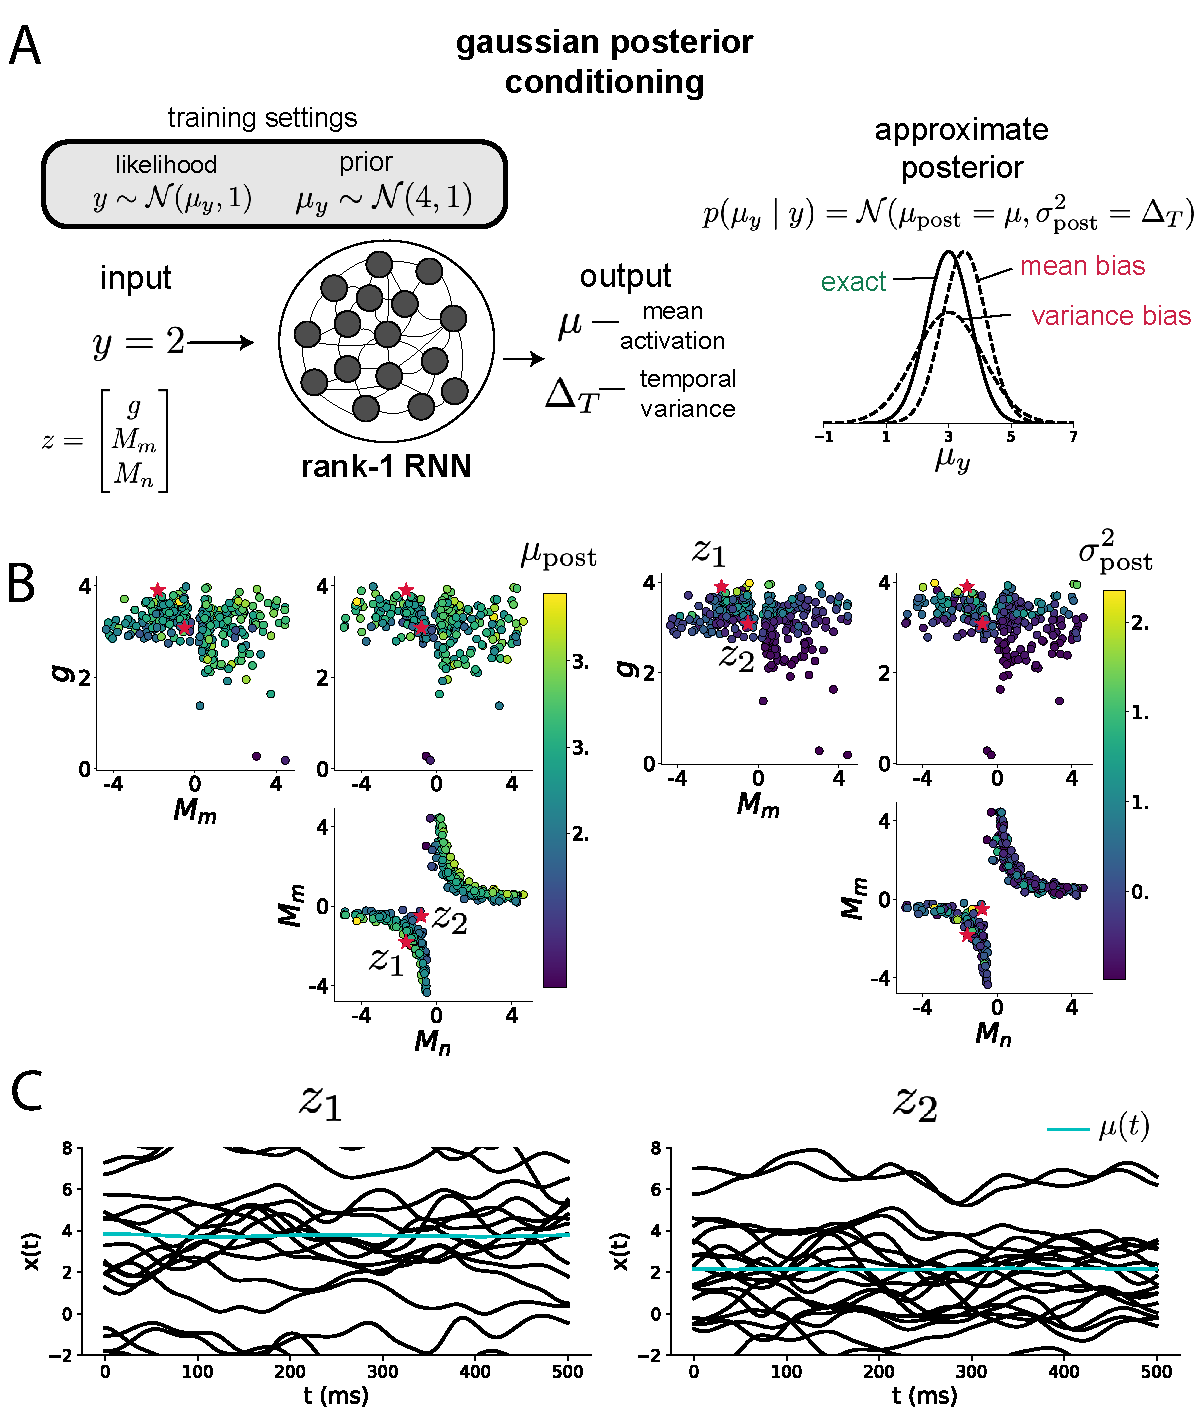
\includegraphics[scale=0.7]{figures/fig5/fig5.pdf}
\end{center}
\caption{Sources of bias in RNN computation.  A. (left) A rank-1 RNN running approximate Bayesian inference on $\mu_y$ assuming a gaussian likelihood variance of 1 and a prior of $\mathcal{N}(4,1)$.  (center) The rank-1 RNN represents the computed Gaussian posterior mean $\mu_{\text{post}}$ and variance $\sigma^2_{\text{post}}$  in its mean activity $\mu$ and its temporal variance $\Delta_T$.  (right) Bias in this computation can come from over- or under-estimating the posterior mean or variance. B. Distribution of rank-1 RNNs executing approximate Bayesian inference.  Samples are colored by (left) posterior mean $\mu_{\text{post}}=\mu$ and (right) posterior variance $\sigma^2_{\text{post}}=\Delta_T$  C. Finite size realizations agree with the DMFT theory.}
\end{figure}

\section{Discussion}
\subsection{EPI is a general tool for theoretical neuroscience} 
Models of biological systems are often comprised of complex nonlinear differential equations, making traditional theoretical analysis and statistical inference intractable. 
In contrast, EPI is capable of learning distributions of parameters in such models producing measurable signatures of computation.
We have demonstrated its utility on biological models (STG), intermediate-level models of interacting genetically- and functionally-defined neuron-types (V1, SC), and the most abstract of models (RNNs).  
We are able to condition both deterministic and stochastic models on low-level emergent properties like firing rates of membrane potentials, as well as high-level cognitive function like Gaussian posterior conditioning.
Technically, EPI is tractable when the emergent property statistics are continuously differentiable with respect to the model parameters, which is very often the case; this emphasizes the general utility of EPI.

In this study, we have focused on applying EPI to low dimensional parameter spaces of models with low dimensional dynamical state.
These choices were made to present the reader with a series of  interpretable conclusions, which is more challenging in high dimensional spaces.
In fact, EPI should scale reasonably to high dimensional parameter spaces, as the underlying technology has produced state-of-the-art performance on high-dimensional tasks such as texture generation \cite{loaiza2017maximum}.
Of course, increasing the dimensionality of the dynamical state of the model makes optimization more expensive, and there is a practical limit there as with any machine learning approach.
For systems with high dimensional state, we recommend using theoretical approaches (e.g. \cite{mastrogiuseppe2018linking}) to reason about reduced parameterizations of such high-dimensional systems.

There are additional technical considerations when assessing the suitability of EPI for a particular modeling question.  
First and foremost, as in any optimization problem, the defined emergent property should always be appropriately conditioned (constraints should not have wildly different units).  
Furthermore, if the program is underconstrained (not enough constraints), the distribution grows (in entropy) unstably unless mapped to a finite support.  
If overconstrained, there is no parameter set producing the emergent property, and EPI optimization will fail (appropriately).
Next, one should consider the computational cost of the gradient calculations. 
In the best circumstance, there is a simple, closed form expression (e.g. Section \ref{methods_2DLDS}) for the emergent property statistic given the model parameters.  
On the other end of the spectrum, many forward simulation iterations may be required before a high quality measurement of the emergent property statistic is available  (e.g. Section \ref{methods_STG}).  In such cases, optimization will be expensive.

\subsection{Novel hypotheses from EPI} 
Machine learning has played an effective, multifaceted role in neuroscientific progress. 
Primarily, it has revealed structure in large-scale neural datasets \cite{kass2001spike, brown1998statistical, paninski2004maximum, byron2009gaussian, latimer2015single, duncker2019learning} (see review, \cite{paninski2018neural}).  
Secondarily, trained algorithms of varying degrees of biological relevance are beginning to be viewed as fully-observable computational systems comparable to the brain \cite{ sussillo2013opening, richards2019deep}.  

For example, consider the fact that we do not fully understand the four-dimensional models of V1 \cite{litwin2016inhibitory}.  
Because analytical approaches to studying nonlinear dynamical systems become increasingly complicated when stepping from two-dimensional to three- or four-dimensional systems in the absence of restrictive simplifying assumptions \cite{strogatz1994nonlinear}, it is unsurprising that this model has been a challenge. 
In Section \ref{results_V1}, we showed that EPI was far more informative about neuron-type input responsivity than the predictions afforded through analysis.
By flexibly conditioning this V1 model on different emergent properties, we performed an exploratory analysis of a \emph{model} rather than a dataset, which generated and proved out a set of testable predictions. 
%Thus, we promote the use of EPI to gain desired model insights.

Of course, exploratory analyses can also be directed.  For example,  when interested in model changes during learning, one can use EPI to condition as we did in Section \ref{results_SC}.
This analysis identified experimentally testable predictions (proved out \textit{in-silico}) of changes in connectivity in SC throughout learning.
Precisely, we predict that an initial reduction in side mode eigenvalue, and a steady increase in task mode eigenvalue will take place, during learning, in the effective connectivity matrices of learning rats.
%While experimentally testable predictions are highly valuable, sometimes it is prohibitively challenging to design a biologically realistic model of a neural computation.
%Thusly, RNNs have become an increasingly popular tool in systems neuroscience research.  
%The scientific philosophy is as follows: optimize an RNN to execute a task from behavioral neuroscience, compare the activity of this optimized system to brain activity from a model organism doing the same task, and leverage the full observability of the trained RNN to generate hypotheses of the neural mechanisms of computation.  
%While fixed point identification and jacobian measurement yield intuitive, consistent portraits of the implemented computational algorithm \cite{universality2019Maheswaranathan}, there is dizzying degeneracy in the RNN connectivity matrix with respect to these characterizations.  
%Since neural activity generally lies on a low dimensional manifold \cite{gao2015simplicity}, we may attain an understanding of the neural mechanisms at play in cortical processing by working in a reduced, interpretable parameter setting of these powerfully general models \cite{doya1993universality}.

In our final analysis, we present a novel procedure for doing statistical inference on interpretable parameterizations of RNNs executing simple tasks .  This methodology relies on recently extended theory of responses in random neural networks with minimal structure \cite{mastrogiuseppe2018linking}. With this methodology, we can finally open the probabilistic model selection toolkit reasoning about the connectivity of RNNs solving tasks.

%\item Link conditioning on task execution with work done today with RNNs.  Although there seems to be consistency across RNN architectures \cite{universality2019Maheswaranathan}, basically we're training overparameterized models with regression, and get a distribution (we have no prob treatment of). Emphasize utility of low-dim interpretable parameterizations. RNNs are particularly useful, when an interpretable model can not easily be designed to execute a task/behavior of interest. Other relevant work \cite{zhao2016interpretable, duncker2019learning}.
%Elaborate on idea of conditioning on flexibly defined statistics i.e. emergent properties. Emphasize how this is practical.  Link to sufficient statistics, esp. commonly used in phenom models like spike counts etc.
%A paragraph on bridging large scale recordings with theory.


\bibliography{NN2019}
\bibliographystyle{unsrt}

\appendix

\section{Methods}

\subsection{Emergent property inference (EPI)}\label{methods_EPI}
Emergent property inference (EPI) learns distributions of theoretical model parameters that produce emergent properties of interest.  EPI combines ideas from likelihood-free variational inference \cite{tran2017hierarchical} and maximum entropy flow networks \cite{loaiza2017maximum}.  A maximum entropy flow network is used as a deep probability distribution for the parameters, while these samples often parameterize a differentiable model simulator, which may lack a tractable likelihood function.

Consider model parameterization $z$ and data $x$ generated from some theoretical model simulator represented as $p(x \mid z)$, which may be deterministic or stochastic.  Theoretical models usually have known sampling procedures for simulating activity given a circuit parameterization, yet often lack an explicit likelihood function due to the nonlinearities and dynamics. With EPI, a distribution on parameters $z$ is learned, that yields an emergent property of interest $\mathcal{B}$,
\begin{equation}
\mathcal{B} \leftrightarrow E_{z \sim q_\theta}\left[ E_{x\sim p(x \mid z)}\left[T(x)\right] \right] = \mu
\end{equation}
by making an approximation $q_\theta(z)$ to $p(z \mid \mathcal{B})$ (see Section \ref{methods_VI}).  So, over the DSN distribution $q_\theta(z)$ of model $p(x \mid z)$ for behavior $\mathcal{B}$, the emergent properties $T(x)$ are constrained in expectation to $\mu$.

 In deep probability distributions, a simple random variable $w \sim p_0$ is mapped deterministically via a function $f_\theta$ parameterized by a neural network to the support of the distribution of interest where $z = f_{\theta}(\omega) = f_l(..f_1(\omega))$.  Given a theoretical model $p(x \mid z)$ and some behavior of interest $\mathcal{B}$, the deep probability distributions are trained by optimizing the neural network parameters $\theta$ to find a good approximation $q_{\theta}^*$ within the deep variational family $Q$ to $p(z \mid \mathcal{B})$.

In most settings (especially those relevant to theoretical neuroscience) the likelihood of the behavior with respect to the model parameters $p(T(x) \mid z)$ is unknown or intractable, requiring an alternative to stochastic gradient variational Bayes \cite{kingma2013auto} or black box variational inference\cite{ranganath2014black}.  These types of methods called likelihood-free variational inference (LFVI, \cite{tran2017hierarchical}) skate around the intractable likelihood function in situations where there is a differentiable simulator. Akin to LFVI, DSNs are optimized with the following objective for a given theoretical model, emergent property statistics $T(x)$, and emergent property constraints $\mu$:

\begin{equation}
\begin{split}
q_\theta^*(z) &= \argmax_{q_\theta \in Q} H(q_\theta(z)) \\
 &  \text{s.t.  } E_{z \sim q_\theta}\left[ E_{x\sim p(x \mid z)}\left[T(x)\right] \right] = \mu \\
 \end{split}
\end{equation}

Optimizing this objective is a technological accomplishment in its own right, the details of which we elaborate in Section \ref{methods_AL_opt}.  Before going through those details, we ground this optimization in a toy example.

\subsubsection{Example: 2D LDS}\label{methods_2DLDS}
To gain intuition for EPI, consider two-dimensional linear dynamical systems, $\tau \dot{x} = Ax$ with 
\[A = \begin{bmatrix} a_1 & a_2 \\ a_3 & a_4 \end{bmatrix}\]
 that produce a band of oscillations. To do EPI with the dynamics matrix elements as the free parameters $z = \left[a_1, a_2, a_3, a_4 \right]$, and fixing $\tau=1$, such that the posterior yields a band of oscillations, the emergent property statistics $T(x)$ are chosen to contain the first- and second-moments of the oscillatory frequency $\Omega$ and the growth/decay factor $d$ of the oscillating system.  To learn the distribution of real entries of $A$ that yield a distribution of $d$ with mean zero with variance $0.25^2$, and oscillation frequency $\Omega$ with mean 1 Hz with variance (0.1Hz)$^2$, then we would select the real part of the complex conjugate eigenvalues $\text{real}(\lambda_1) = d$ (via an arbitrary choice of eigenvalue of the dynamics matrix $\lambda_1$) and the positive imaginary component of one of the eigenvalues $\text{imag}(\lambda_1) = 2 \pi \Omega$ as the emergent property statistics.  Those emergent property statistics are then constrained to
\begin{equation}
 \mu = E \begin{bmatrix} \text{real}(\lambda_1) \\ \text{imag}(\lambda_1) \\ (\text{real}(\lambda_1)-0)^2  \\ (\text{imag}(\lambda_1)-2 \pi \Omega)^2 \end{bmatrix} = \begin{bmatrix} 0.0 \\ 2 \pi \Omega \\ 0.25^2 \\ (2 \pi 0.1)^2 \end{bmatrix}
 \end{equation} 
 
\begin{figure}
\begin{center}
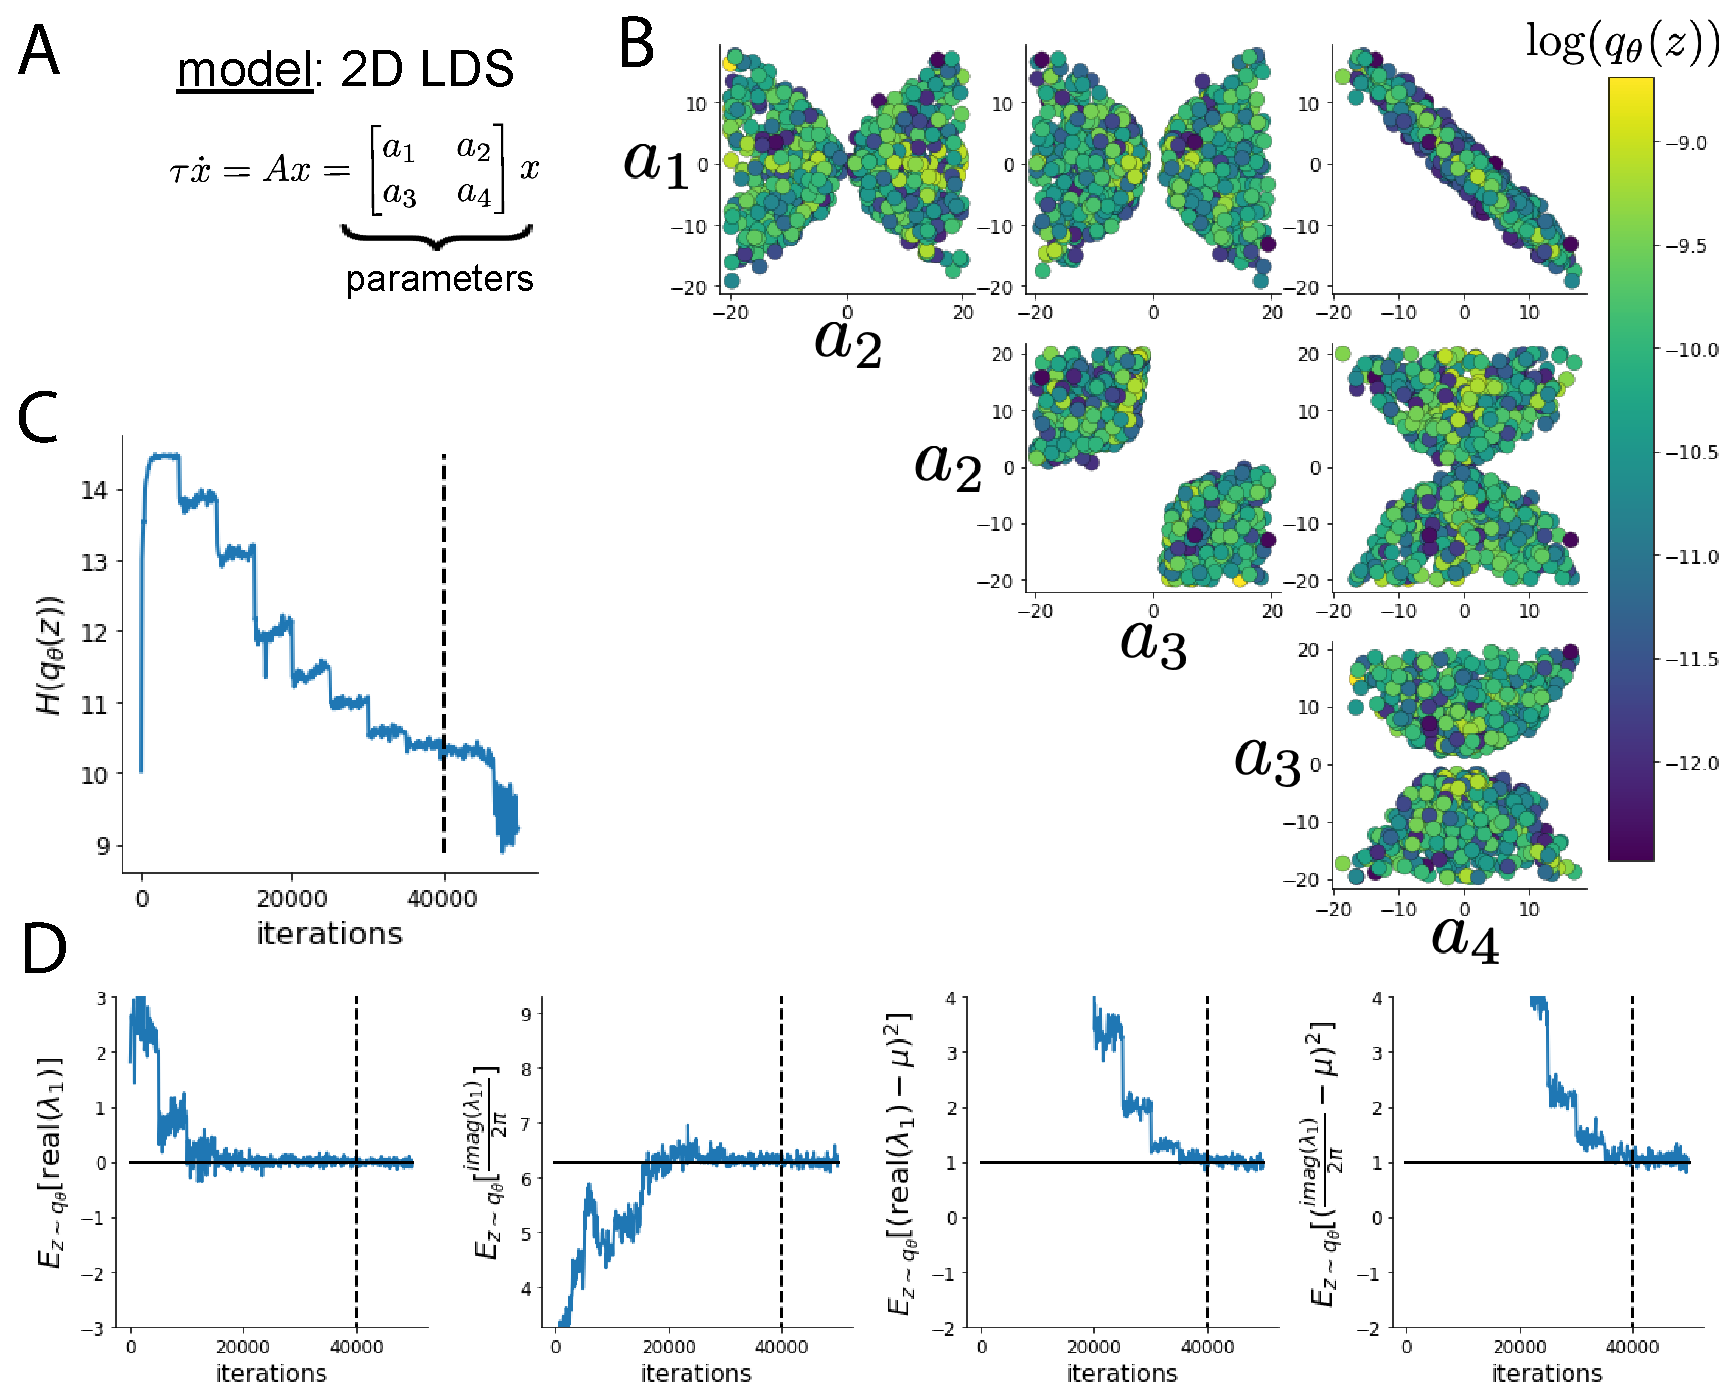
\includegraphics[scale=0.5]{figures/figS2/figS2.pdf}
\end{center}
\begin{flushleft}
Fig. S2: A. Two-dimensional linear dynamical system model, where real entries of the dynamics matrix $A$ are the parameters.  B. The DSN distribution for a 2D LDS with $\tau=1$ that produces an average of 1Hz oscillations with some small amount of variance.  C. Entropy throughout the optimization.  At the beginning of each augmented Lagrangian epoch (5,000 iterations), the entropy dips due to the shifted optimization manifold where emergent property constraint satisfaction is increasingly weighted.  D. Emergent property moments throughout optimization.  At the beginning of each augmented Lagrangian epoch, the emergent property moments move closer to their constraints.
\end{flushleft}
\end{figure}

where $\Omega = 1$Hz.  Unlike the models we study in the paper which calculate $E_{x \sim p(x \mid z)} \left[T(x) \right]$ via forward simulation, we have a closed  form for the eigenvalues of the dynamics matrix.  $\lambda$ can be calculated using the quadratic formula: 
\begin{equation}
\lambda = \frac{(\frac{a_1 + a_4}{\tau}) \pm \sqrt{(\frac{a_1+a_4}{\tau})^2 + 4(\frac{a_2 a_3 - a_1 a_4}{\tau})}}{2}
\end{equation}
where $\lambda_1$ is the eigenvalue of $\frac{1}{\tau}A$ with greatest real part.  Even though $E_{x\sim p(x \mid z)}\left[T(x)\right]$ is calculable directly via a closed form function and does not require simulation, we cannot derive the distribution $q^*_\theta$ directly.  This is due to the formally hard problem of the backward mapping: finding the natural parameters $\eta$ from the mean parameters $\mu$ of an exponential family distribution \cite{wainwright2008graphical}.  Instead, we can use EPI to learn the linear system parameters producing such a band of oscillations (Fig. S2B). 

Even this relatively simple system has nontrivial (though intuitively sensible) structure in the parameter distribution.  To validate our method (further than that of the underlying technology on a ground truth solution \cite{loaiza2017maximum}) we can analytically derive the contours of the probability density from the emergent property statistics and values (Fig. S3).  In the $a_1-a_4$ plane, is a black line at $\text{real}(\lambda_1) = \frac{a_1 + a_4}{2} = 0$, a dotted black line at
the standard deviation $\text{real}(\lambda_1) = \frac{a_1 + a_4}{2} \pm 1$, and a grey line at twice the standard deviation
$\text{real}(\lambda_1) = \frac{a_1 + a_4}{2} \pm 2$ (Fig. S3A). Here the lines denote the set of solutions at fixed behaviors, which overlay the posterior obtained through EPI.  The learned DSN distribution precisely reflects the desired statistical constraints and model degeneracy in the sum of
$a_1$ and $a_4$. Intuitively, the parameters equivalent with respect to emergent property statistic $\text{real}(\lambda_1)$ have similar log densities.

To explain the structure in the bimodality of the DSN posterior, we can look at the imaginary component of $\lambda_1$.  When $\text{real}(\lambda_1) = \frac{a_1 + a_4}{2} = 0$, we have
\begin{equation}
\text{imag}(\lambda_1) = \begin{cases}
                             \sqrt{\frac{a_1 a_4 - a_2 a_3}{\tau}},  & \text{if } a_1 a_4 < a_2 a_3 \\
                             0 & \text{otherwise } \\
                         \end{cases} 
\end{equation}

When $\tau=1$ and $a_1 a_4 > a_2 a_3$ (center of distribution above), we have the following equation for the other two dimensions:

\begin{equation}
\text{imag}(\lambda_1)^2 = a_1 a_4 - a_2 a_3
\end{equation}

Since we constrained $E_{q_\theta}\left[\text{imag}(\lambda)\right] = 2 \pi$ (with $\omega=1$), we can plot contours of the equation $\text{imag}(\lambda_1)^2 = a_1 a_4 - a_2 a_3 = (2 \pi)^2$ for various $a_1 a_4$ (Fig. S3A). If $\sigma_{1,4} = E_{q_\theta}(|a_1 a_4 - E_{q_\theta}[a_1 a_4]|)$, then we plot the contours as $a_1 a_4 = 0$ (black), $a_1 a_4 = -\sigma_{1,4}$ (black dotted), and $a_1 a_4 = -2\sigma_{1,4}$ (grey dotted) (Fig. S3B). This validates the curved structure of the inferred distribution learned through EPI.  We take steps in negative standard deviation of $a_1 a_4$ (dotted and gray lines), since there are few positive values $a_1 a_4$ in the posterior.  Subtler model-behavior combinations will have even more complexity, further motivating the use of EPI for understanding these systems.  Indeed, we sample a distribution of systems oscillating near 1Hz (Fig. S4).

\begin{figure}
\begin{center}
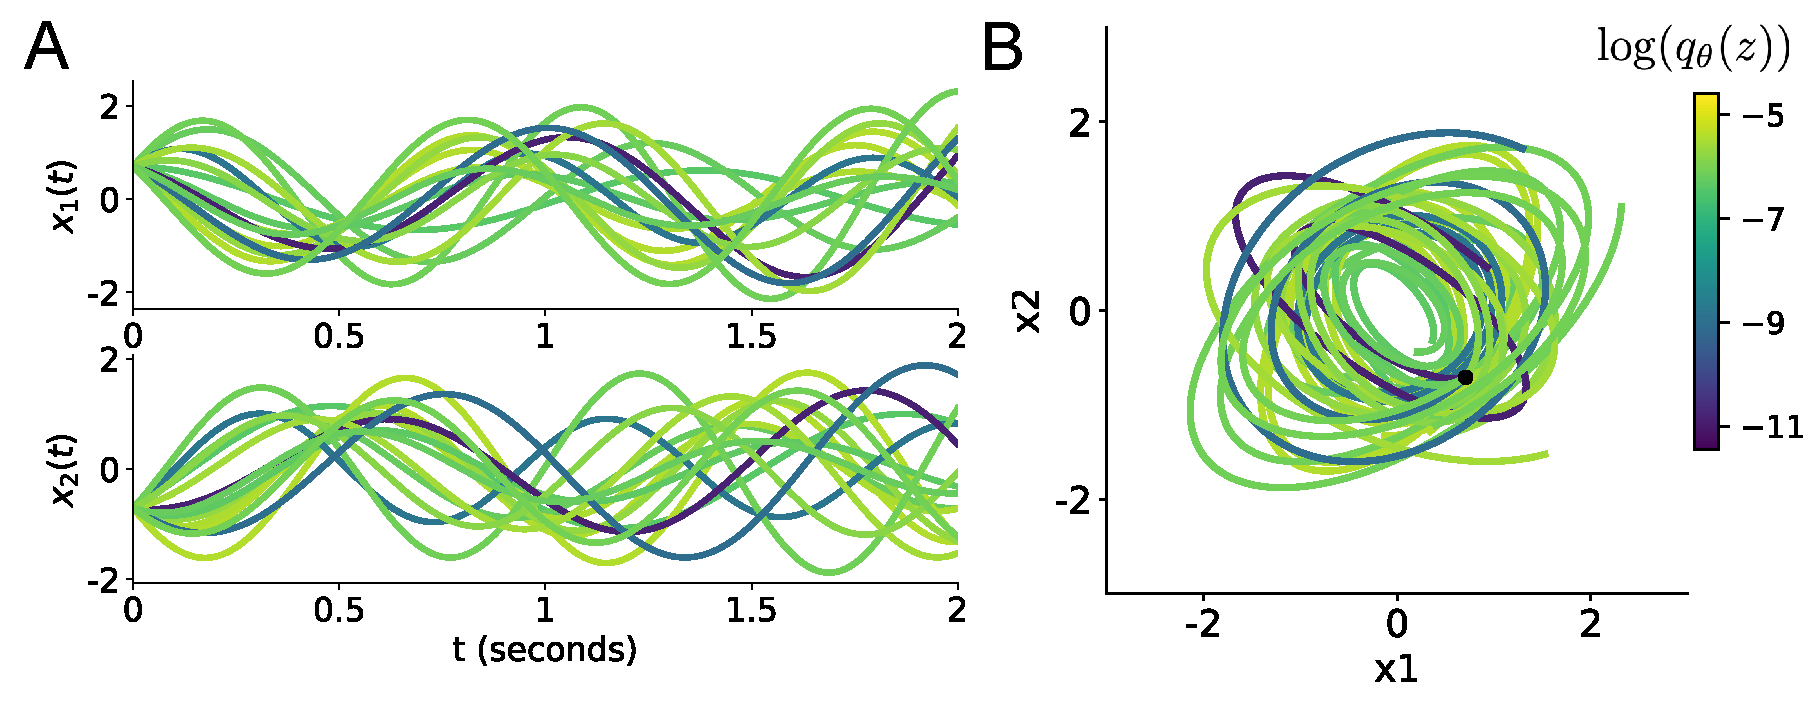
\includegraphics[scale=0.5]{figures/figS3/figS3.pdf}
\end{center}
\begin{flushleft}
Fig. S3: A. Probability contours in the $a_1-a_4$ plane can be derived from the relationship to emergent property statistic of growth/decay factor. B. Probability contours in the $a_2-a_3$ plane can be derived from relationship to the emergent property statistic of oscillation frequency.
\end{flushleft}
\end{figure}

\begin{figure}
\begin{center}
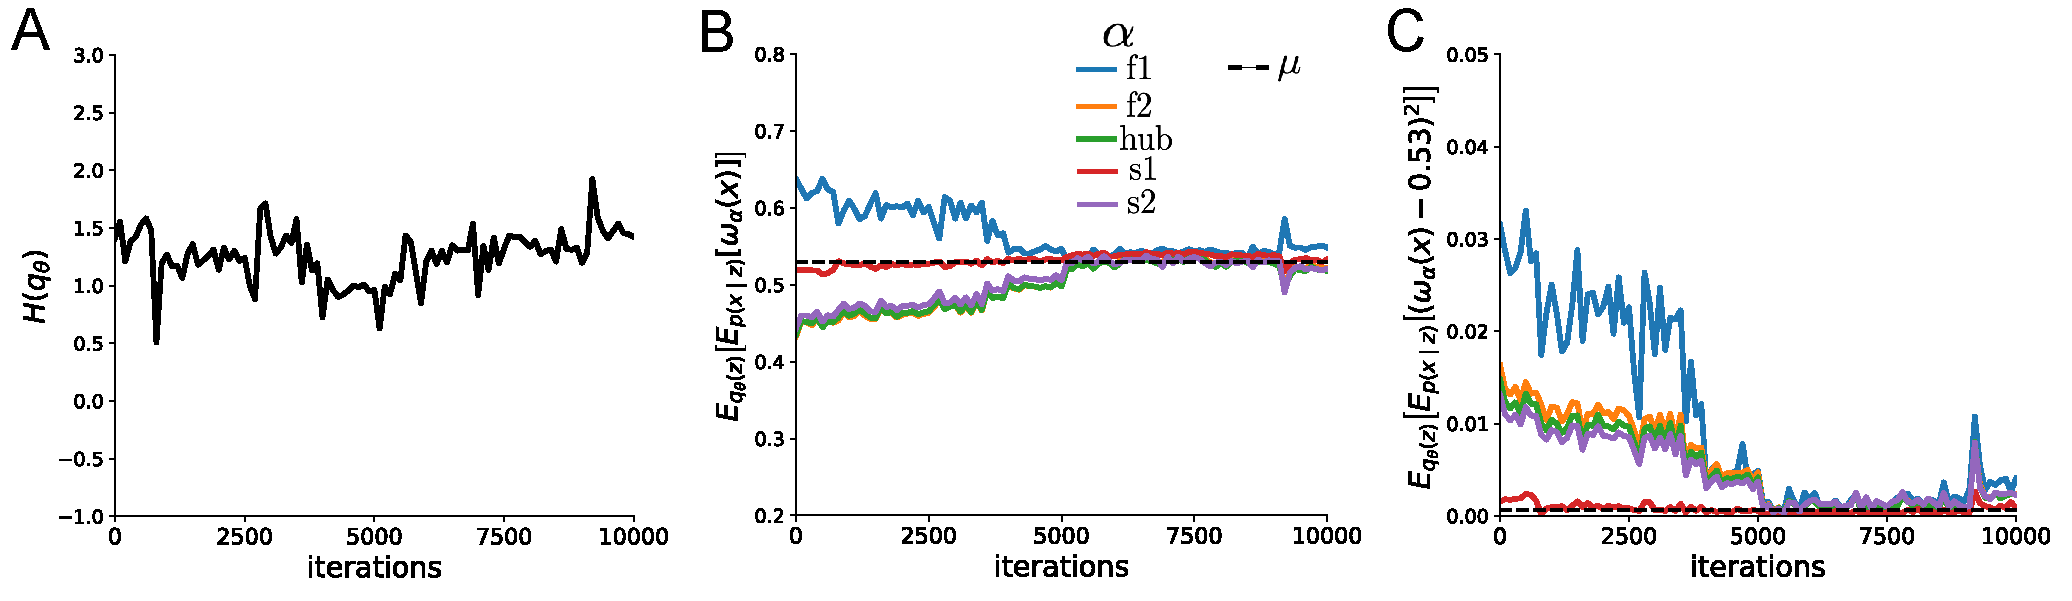
\includegraphics[scale=0.5]{figures/figS4/figS4.pdf}
\end{center}
\begin{flushleft}
Fig. S4: Sampled dynamical system trajectories from the EPI distribution.  Each trajectory is initialized at $x(0) = \begin{bmatrix} \frac{\sqrt{2}}{2} & -\frac{\sqrt{2}}{2} \end{bmatrix}$.
\end{flushleft}
\end{figure}

\subsubsection{Augmented Lagrangian optimization}\label{methods_AL_opt}
To optimize $q_\theta(z)$ in equation 1, the constrained optimization is performed using the augmented Lagrangian method.  The following objective is minimized:
\begin{equation}
L(\theta; \alpha, c) = -H(q_\theta) + \alpha^\top \delta(\theta) + \frac{c}{2}||\delta(\theta)||^2
\end{equation}
where $\delta(\theta) = E_{z \sim q_\theta}\left[ E_{x\sim p(x \mid z)}\left[T(x) - \mu \right] \right]$, $\alpha \in \mathcal{R}^m$ are the Lagrange multipliers and $c$ is the penalty coefficient.  For a fixed $(\alpha, c)$, $\theta$ is optimized with stochastic gradient descent.  A low value of $c$ is used initially, and increased during each augmented Lagrangian epoch -- a period of optimization with fixed $\alpha$ and $c$ for a given number of stochastic optimization iterations. Similarly, $\alpha$ is tuned each epoch based on the constraint violations.  For the linear 2-dimensional system (Fig. S2C) optimization hyperparameters are initialized to $c_1 = 10^{-4}$ and $\alpha_1 = 0$.  The penalty coefficient is updated based on a hypothesis test regarding the reduction in constraint violation.  The p-value of $E[||\delta(\theta_{k+1})||] > \gamma E[||\delta(\theta_{k})||]$ is computed, and $c_{k+1}$ is updated  to $\beta c_k$ with probability $1-p$.  Throughout the project, $\beta = 4.0$ and $\gamma = 0.25$ is used.  The other update rule is $\alpha_{k+1} = \alpha_k + c_k \frac{1}{n} \sum_{i=1}^n (T(x^{(i)}) - \mu)$.  In this example, each augmented Lagrangian epoch ran for 2,000 iterations.  We consider the optimization to have converged when a null hypothesis test of constraint violations being zero is accepted for all constraints at a significance threshold 0.05.  This is the dotted line on the plots below depicting the optimization cutoff of EPI optimization for the 2-dimensional linear system.  If the optimization is left to continue running, entropy usually decreases, and structural pathologies in the distribution may be introduced.

The intention is that $c$ and $\alpha$ start at values encouraging entropic growth early in optimization.  Then, as they increase in magnitude with each training epoch, the constraint satisfaction terms are increasingly weighted, resulting in a decrease in entropy.  Rather than using a naive initialization, before EPI, we optimize the deep probability distribution parameters to generate samples of an isotropic Gaussian of a selected variance, such as 1.0 for the 2D LDS example.  This provides a convenient starting point, whose level of entropy is controlled by the user.



\subsubsection{Normalizing flows}\label{methods_NF}
Since we are optimizing parameters $\theta$ of our deep probability distribution with respect to the entropy, we will need to take gradients with respect to the log-density of samples from the deep probability distribution.

\begin{equation}
H(q_\theta(z)) = \int - q_\theta(z) \log(q_\theta(z)) dz = E_{z \sim q_\theta}\left[-\log(q_\theta(z)) \right] = E_{\omega \sim q_0}\left[-\log(q_\theta(f_\theta(\omega))) \right]
\end{equation}
\begin{equation}
\nabla_\theta H(q_\theta(z)) = E_{\omega \sim q_0}\left[- \nabla_\theta \log(q_\theta(f_\theta(\omega))) \right]
\end{equation}

Deep probability models typically consist of several layers of fully connected neural networks.  When each neural network layer is restricted to be a bijective function, the sample density can be calculated using the change of variables formula at each layer of the network.  For $z' = f(z)$,

\begin{equation}
q(z') = q(f^{-1}(z')) \left| \det \frac{\partial f^{-1}(z')}{\partial z'} \right| = q(z) \left| \det \frac{\partial f(z)}{\partial z} \right|^{-1}
\end{equation}

However, this computation has cubic complexity in dimensionality for fully connected layers.  By restricting our layers to normalizing flows \cite{rezende2015variational} -- bijective functions with fast log determinant jacobian computations, we can tractably optimize deep generative models with objectives that are a function of sample density, like entropy. Most of our analyses use real NVP \cite{dinh2017density}, which have proven effective in our architecture searches, and have the advantageous features of fast sampling and fast density evaluation.

\subsubsection{Related work}\label{methods_related_work}
(To come)\\


\subsubsection{Emergent property inference as variational inference in an exponential family}\label{methods_VI}
(To come) \\
%Consider the goal of doing variational inference (VI) in with an exponential family posterior distribution $p(z \mid x)$.  We'll use the following abbreviated notation to collect the base measure and sufficient statistics into $\tilde{T}(z)$ and likewise concatenate a 1 onto the end of the natural parameter $\tilde{\eta}(x)$.  The log normalizing constant $A(\eta(x))$ will remain unchanged.
%\begin{equation}
%\begin{split}
%p(z \mid x) = b(z) \exp{\left( \eta(x)^\top T(z) - A(\eta(x)) \right)} = \exp{\left( \begin{bmatrix} \eta(x) \\ 1 \end{bmatrix}^\top \begin{bmatrix} T(z) \\ b(z) \end{bmatrix} - A(\eta(x)) \right)} \\= \exp{\left(\tilde{\eta(x)}^\top \tilde{T}(z) - A(\eta(x)) \right)} 
%\end{split}
%\end{equation}
%VI looks with an exponential family posterior distribution uses optimization to minimize the following divergence \cite{blei2017variational}:
%\begin{equation}
%q_\theta^* = \argmin_{q_\theta \in Q} KL(q_\theta \mid \mid p(z \mid x))
%\end{equation}
%$q_\theta(z)$ is the variational approximation to the posterior with variational parameters $\theta$.  We can write this KL divergence in terms of entropy of the variational approximation.
%\begin{equation}
%KL(q_\theta \mid \mid p(z \mid x)) = E_{z \sim q_\theta} \left[ \log (q_\theta(z)) \right] - E_{z \sim q_\theta} \left[ \log (p(z \mid x)) \right]
%\end{equation}
%\begin{equation}
% = -H(q_\theta) - E_{z \sim q_\theta} \left[ \tilde{\eta}(x)^\top  \tilde{T}(z) - A(\eta(x)) \right]
%\end{equation}
%As far as the variational optimization is concerned, the log normalizing constant is independent of $q_\theta(z)$, so it can be dropped. 
%\begin{equation}
 %\argmin_{q_\theta \in Q} KL(q_\theta \mid \mid p(z \mid x)) =  \argmin_{q_\theta \in Q} -H(q_\theta) - E_{z \sim q_\theta} \left[ \tilde{\eta}(x)^\top  \tilde{T}(z) \right]
% \end{equation}
% Further, we can write the objective in terms of the first moment of the sufficient statistics $\mu = E_{z \sim p(z \mid x)}\left[T(z) \right]$.
% \begin{equation}
%=  \argmin_{q_\theta \in Q} -H(q_\theta) - E_{z \sim q_\theta} \left[ \tilde{\eta}(x)^\top \left(  \tilde{T}(z) -\mu \right) \right] + \tilde{\eta(x)}^\top \mu
% \end{equation}
%  \begin{equation}
%=  \argmin_{q_\theta \in Q} -H(q_\theta) - E_{z \sim q_\theta} \left[ \tilde{\eta}(x)^\top \left(  \tilde{T}(z) -\mu \right) \right]
% \end{equation}

%In emergent property inference (EPI), we're solving the following problem.
%\begin{equation}
%q_\theta^*(z) y= \argmax_{q_\theta \in Q} H(q_\theta(z)),   \text{  s.t.  } E_{z \sim q_\theta}\left[ E_{x\sim p(x \mid z)}\left[T(x)\right] \right] = \mu
%\end{equation}
%The lagrangian objective is
%\begin{equation}
%q_\theta^* = \argmin_{q_\theta \in Q} - H(q_\theta) + \alpha^\top \left(E_{z \sim q_\theta} \left[\tilde{T}(z) \right] - \mu \right)
%\end{equation}

%As the lagrangian optimization proceeds, $\alpha$ should converge to $\tilde{\eta}(x))$ through its adaptations in each epoch.  More formally, $\tilde{\eta}(x) \leftrightarrow \tilde{\eta}(\mu)$ is referred to as the backward mapping, and is formally hard to identify \cite{wainwright2008graphical}.  Since this backward mapping is deterministic, conceptually, we can replace $p(z \mid x)$ with $p(z \mid \mu)$.  More commonly, we write $p(z \mid \mathcal{B})$ for clarity where $\mathcal{B}$ more explicitly captures the moment constraints of the sufficient statistics.

\subsection{Theoretical models}\label{methods_theoretical_models}
In this study, we used emergent property inference to examine several models relevant to theoretical neuroscience.  Here, we provide the details of each model  and the related analyses.

\subsubsection{Stomatogastric ganglion}\label{methods_STG}
Each neuron's membrane potential $x_m(t)$ is the solution of the following differential equation.
\begin{equation} C_m \frac{dx_m}{dt} = - \left[ h_{leak}(x; z) + h_{Ca}(x; z) + h_K(x; z) + h_{hyp}(x; z) + h_{elec}(x; z) + h_{syn}(x; z)\right] 
\end{equation} 

The membrane potential of each neuron is affected by the leak, calcium, potassium, hyperpolarization,
electrical and synaptic currents, respectively.  The capacitance of the cell membrane was set to $C_m = 1nF$. Each current is a function of the neuron's membrane potential $x_m$ and the parameters of the circuit such as  $g_{el}$ and $g_{syn}$, whose effect on the circuit is considered in the motivational example of EPI in Fig. 1.  Specifically, the currents are the difference in the neuron's membrane potential and that current type's reversal potential multiplied by a conductance:
\begin{equation}  h_{leak}(x; z) = g_{leak} (x_m - V_{leak}) 
\end{equation} 
\begin{equation}  h_{elec}(x; z) = g_{el} (x_m^{post} - x_m^{pre})
\end{equation} 
\begin{equation}  h_{syn}(x; z) = g_{syn} S_\infty^{pre} (x_m^{post} - V_{syn}) \end{equation} 
\begin{equation}  h_{Ca}(x; z) = g_{Ca} M_\infty (x_m - V_{Ca}) 
\end{equation} 
\begin{equation}  h_K(x; z) = g_K N (x_m - V_K) 
\end{equation} 
\begin{equation}  h_{hyp}(x; z) = g_h H(x_m - V_{hyp})
\end{equation} 
The reversal potentials were set to $V_{leak} = -40mV$, $V_{Ca} = 100mV$, $V_K = -80mV$, $V_{hyp} = -20mV$, and $V_{syn} = -75mV$.  The other conductance parameters were fixed to $g_{leak} = 1 \times 10^{-4} \mu S$. $g_{Ca}$, $g_{K}$, and $g_{hyp}$ had different values based on fast, intermediate (hub) or slow neuron.  Fast: $g_{Ca} = 1.9 \times 10^{-2}$, $ g_K = 3.9 \times 10^{-2} $, and $ g_{hyp} = 2.5 \times 10^{-2} $.  Intermediate: $g_{Ca} = 1.7 \times 10^{-2}$, $ g_K = 1.9 \times 10^{-2} $, and $ g_{hyp} = 8.0 \times 10^{-3} $.  Intermediate: $g_{Ca} = 8.5 \times 10^{-3}$, $ g_K = 1.5 \times 10^{-2} $, and $ g_{hyp} = 1.0 \times 10^{-2} $.

Furthermore, the Calcium, Potassium, and hyperpolarization channels have time-dependent gating dynamics dependent on steady-state gating variables $M_\infty$, $N_\infty$ and $H_\infty$, respectively.
\begin{equation}  M_{\infty} = 0.5 \left( 1 + \tanh \left( \frac{x_m - v_1}{v_2} \right) \right) \end{equation}
\begin{equation}  \frac{dN}{dt} = \lambda_N (N_\infty - N)  \end{equation}
\begin{equation}  N_\infty = 0.5 \left( 1 + \tanh \left( \frac{x_m - v_3}{v_4} \right) \right) \end{equation}
\begin{equation}  \lambda_N = \phi_N \cosh \left( \frac{x_m - v_3}{2 v_4} \right) \end{equation}
\begin{equation}  \frac{dH}{dt} = \frac{\left( H_\infty - H \right)}{\tau_h} \end{equation}
\begin{equation}  H_\infty = \frac{1}{1 + \exp \left( \frac{x_m + v_5}{v_6} \right)} \end{equation}
\begin{equation}  \tau_h = 272 - \left( \frac{-1499}{1 + \exp \left( \frac{-x_m + v_7}{v_8} \right)} \right) \end{equation}
where we set $v_1 = 0mV$, $v_2  = 20mV$, $v_3 = 0mV$, $v_4 = 15mV$, $v_5 = 78.3mV$,
$v_6 = 10.5mV$, $v_7 = -42.2mV$, $v_8 = 87.3mV$, $v_9 = 5mV$, and $v_{th} = -25mV$.  These are the same parameter values used in \cite{gutierrez2013multiple}.

Finally, there is a synaptic gating variable as well:
\begin{equation} S_\infty = \frac{1}{1 + \exp \left( \frac{v_{th} - x_m}{v_9} \right)} 
\end{equation}
When the dynamic gating variables are considered, this is actually a 15-dimensional nonlinear dynamical system.

In order to measure the frequency of the hub neuron during EPI, the STG model was simulated for $T = 500$ time steps of $dt = 25ms$.  In EPI, since gradients are taken throught the simulation process, the number of time steps are kept as modest if possible. The chosen $dt$ and $T$ were the most computationally convenient choices yielding accurate frequency measurement.

Our original approach to measuring frequency was to take the max of the fast Fourier transform (FFT) of the simulated time series.  There are a few key considerations here.  One is resolution in frequency space.  Each FFT entry will correspond to a signal frequency of $\frac{F_s k}{N}$, where N is the number of samples used for the FFT, $F_s = \frac{1}{dt}$, and $k \in \left[0, 1, ..., N-1\right]$.  Our resolution is improved by increasing $N$ and decreasing $dt$.  Increasing N = T-b, where $b$ is some fixed number of buffer burn-in initialization samples, necessitates an increase in simulation time steps $T$, which directly increases computational cost.  Increasing $F_s$ (decreasing $dt$) increases system approximation accuracy, but requires more time steps before a full cycle is observed.  At the level of $dt = 0.025$, thousands of temporal samples were required for resolution of .01Hz.  These challenges in frequency resolution with the discrete Fourier transform motivated the use of an alternative basis of complex exponentials.  Instead, we used a basis of complex exponentials with frequencies from 0.0-1.0 Hz at 0.01Hz resolution, $\Phi = \left[ 0.0, 0.01, ..., 1.0 \right]^\top$

Another consideration was that the frequency spectra of the hub neuron has several peaks.  This was due to high-frequency sub-threshold activity. The maximum frequency was often not the firing frequency.  Accordingly, subthreshold activity was set to zero, and the whole signal was low-pass filtered with a moving average window of length 20.  The signal was subsequently mean centered.  After this pre-processing, the maximum frequency in the filter bank accurately reflected the firing frequency.

Finally, to differentiate through the maximum frequency identification step, we used a sum-of-powers normalization strategy: Let $\mathcal{X}_i \in \mathcal{C}^{|\Phi|}$ be the complex exponential filter bank dot products with the signal $x_i \in \mathcal{R}^{N}$, where $i \in \{ \text{f1}, \text{f2}, \text{hub}, \text{s1}, \text{s2} \}$.  The ``frequency identification" vector is 
\begin{equation}
u_i = \frac{|\mathcal{X}_i|^\alpha}{\sum_{k=1}^N |\mathcal{X}_i(k)|^\alpha}
\end{equation}
The frequency is then calculated as $\Omega_i = u_i^\top \Phi$ with $\alpha = 100$.

Network syncing, like all other emergent properties in this work, are defined by the emergent property statistics and values.  The emergent property statistics are the first- and second-moments of the firing frequencies. The first moments are set to 0.55Hz, while the second moments are set to 0.025Hz$^2$.
\begin{equation}
E \begin{bmatrix} \Omega_{\text{f1}} \\ \Omega_{\text{f2}} \\ \Omega_{\text{hub}} \\ \Omega_{\text{s1}} \\ \Omega_{\text{s2}} \\ (\Omega_{\text{f1}} - 0.55)^2 \\ (\Omega_{\text{f2}} - 0.55)^2 \\ (\Omega_{\text{hub}} - 0.55)^2 \\ (\Omega_{\text{s1}} - 0.55)^2 \\ (\Omega_{\text{s2}} - 0.55)^2  \end{bmatrix} = \begin{bmatrix} 0.55 \\ 0.55 \\ 0.55 \\ 0.55 \\ 0.55 \\ 0.025^2 \\ 0.025^2 \\ 0.025^2 \\ 0.025^2 \\ 0.025^2 \end{bmatrix}
\end{equation}
For EPI in Fig 2C, we used a real NVP architecture with two coupling layers.  Each coupling layer had two hidden layers of 10 units each, and we mapped onto a support of $z \in \left[ \begin{bmatrix} 0 \\ 0 \end{bmatrix}, \begin{bmatrix} 10 \\ 8 \end{bmatrix} \right]$  We have shown the EPI optimization that converged with maximum entropy across 2 random seeds and augmented Lagrangian coefficient initializations of $c_0$=0, 2, and 5.

\subsubsection{Primary visual cortex}\label{methods_V1}
The dynamics of each neural populations average rate
$x = \begin{bmatrix} x_E \\ x_P \\ x_S \\ x_V \end{bmatrix}$
are given by:
\begin{equation}
\tau \frac{dx}{dt} = -x + [W x+ h]_+^n
\end{equation}

Some neuron-types largely lack synaptic projections to other neuron-types \cite{pfeffer2013inhibition}, and it is popular to only consider a subset of the effective connectivities \cite{litwin2016inhibitory}.
\begin{equation}
W = \begin{bmatrix} W_{EE} & W_{EP} & W_{ES} & 0 \\
                                W_{PE} & W_{PP} & W_{PS} & 0 \\
                                W_{SE} & 0 & 0 & W_{SV} \\
                                W_{VE} & W_{VP} &  W_{VS} &  0 \end{bmatrix}
\end{equation}

By consolidating information from many experimental datasets, Billeh et al. \cite{billeh2019systematic} produce estimates of the synaptic strength (in mV)
\begin{equation}
M = \begin{bmatrix} 0.36 & 0.48 & 0.31 & 0.28 \\
1.49 & 0.68 & 0.50 & 0.18 \\
0.86 & 0.42 & 0.15 & 0.32 \\
1.31 & 0.41 & 0.52 & 0.37 \end{bmatrix}
\end{equation}
and connection probability
\begin{equation}
C = \begin{bmatrix} 0.16 & 0.411 & 0.424 &  0.087 \\
0.395 & .451 & 0.857 & 0.02 \\
0.182 & 0.03 & 0.082 & 0.625 \\
0.105 & 0.22 & 0.77 & 0.028 \end{bmatrix}
\end{equation}

Multiplying these connection probabilities and synaptic efficacies gives us an effective connectivity matrix:
\begin{equation}
W_{\text{full}} = C \odot M = \begin{bmatrix} 0.16 & 0.411 & 0.424 &  0.087 \\
0.395 & .451 & 0.857 & 0.02 \\
0.182 & 0.03 & 0.082 & 0.625 \\
0.105 & 0.22 & 0.77 & 0.028 \end{bmatrix}
\end{equation}

From use the entries of this full effective connectivity matrix that are not considered to be ineffectual.

We look at how this four-dimensional nonlinear dynamical model of V1 responds to different inputs, and compare the predictions of the linear response to the approximate posteriors obtained through EPI.  The input to the system is the sum of a baseline input $b = \begin{bmatrix} 1 & 1 & 1 & 1 \end{bmatrix}^\top$ and a differential input $dh$:
\begin{equation}
h = b + dh
\end{equation}
All simulations of this system had $T=100$ time points, a time step $dt = 5$ms, and time constant $\tau = 20$ms.  And the system was initialized to a random draw $x(0)_i \sim \mathcal{N}(1, 0.01)$.

We can describe the dynamics of this system more generally by
\begin{equation}
\dot{x}_i = -x_i + f(u_i)
\end{equation}
where the input to each neuron is
\begin{equation}
u_i = \sum_j W_{ij} x_j + h_i
\end{equation}
Let $F_{ij} = \gamma_i \delta(i,j)$, where $\gamma_i = f'(u_i)$.  Then, the linear response is
\begin{equation}
\frac{dx_{ss}}{dh} = F(W\frac{dx_{ss}}{dh} + I)
\end{equation}
which is calculable by
\begin{equation}
\frac{dx_{ss}}{dh} = (F^{-1} - W)^{-1}
\end{equation}

The emergent property we considered was the first and second moments of the change in rate $dx$ between the baseline input $h= b$ and $h = b + dh$.  We use the following notation to indicate that the emergent property statistics were set to the following values:
\begin{equation}
\mathcal{B}(\alpha, y) \leftrightarrow 
E \begin{bmatrix} dx_{\alpha,ss} \\ (dx_{\alpha,ss} - y)^2 \end{bmatrix} = \begin{bmatrix} y \\ 0.01^2 \end{bmatrix}
\end{equation}

In the final analysis for this model, we sweep the input one neuron at a time away from the mode of each inferred distributions $dh^* = z^* = \argmax_{z} \log q_\theta(z \mid \mathcal{B}(\alpha, 0.1)$.
The differential responses $dx_{\alpha,ss}$ are examined at perturbed inputs  $h = b + dh^* + \Delta h_\alpha u_\alpha$ where $u_\alpha$ is a unit vector in the dimension of $\alpha$ and $\Delta h_\alpha \in \left[-15,15\right]$.

For each $\mathcal{B}(\alpha, y)$ with $\alpha \in \{E, P, S, V\}$ and $y \in \{0.1, 0.5\}$, we ran EPI with five different random initial seeds using an architecture of four coupling layers, each with two hidden layers of 10 units.  We set $c_0 = 10^5$.  The support of the learned distribution was restricted to $z_i \in \left[-5, 5\right]$.


\subsubsection{Superior colliculus}\label{methods_SC}
There are four total units: two in each hemisphere corresponding to the Pro/Contra and Anti/Ipsi populations.  Each unit has an activity ($x_i$) and internal variable ($u_i$) related by
\begin{equation}
x_i(t) =\left(\frac{1}{2}\tanh\left(\frac{v_i(t) - \epsilon}{\zeta}\right)+ \frac{1}{2} \right)
\end{equation}
$\epsilon = 0.05$ and $\zeta = 0.5$ control the position and shape of the nonlinearity, repsectively.

We can order the elements of $x_i$ and $v_i$ into vectors $x$ and $v$ with elements
\begin{equation}
x = \begin{bmatrix} x_{LP} \\ x_{LA} \\ x_{RP} \\ x_{RA} \end{bmatrix} \hspace{2cm} v = \begin{bmatrix} v_{LP} \\ v_{LA} \\ v_{RP} \\ v_{RA} \end{bmatrix}
\end{equation}

 The internal variables follow dynamics:
\begin{equation}
\tau \frac{dv}{dt} = -v + Wx + h + \sigma dB
\end{equation}
with time constant $\tau = 0.09s$ and Gaussian noise $\sigma dB$ controlled by the magnitude of $\sigma=1.0$.  The weight matrix has 8 parameters $sW_P$, $sW_A$, $vW_{PA}$, $vW_{AP}$, $hW_P$, $hW_A$, $dW_{PA}$, and $dW_{AP}$ (Fig. 4B).
\begin{equation}
W = \begin{bmatrix} sW_P & vW_{PA} & hW_P & dW_{PA}  \\ vW_{AP}  & sW_A & dW_{AP}  & hW_A \\ hW_P & dW_{PA}  & sW_P & vW_{PA}  \\ dW_{AP}  & hW_A & vW_{AP}  & sW_A \end{bmatrix}
\end{equation}

The system receives five inputs throughout each trial, which has a total length of 1.8s.
\begin{equation}
h = h_{\text{rule}} + h_{\text{choice-period}} + h_{\text{light}}
\end{equation}

There are rule-based inputs depending on the condition,
\begin{equation}h_{\text{P,rule}}(t) = \begin{cases}
                           I_{\text{P,rule}} \begin{bmatrix} 1 & 0 & 0 & 1 \end{bmatrix}^\top,& \text{if } t\leq 1.2s \\
                            0,              & \text{otherwise}
                         \end{cases}
\end{equation}
\begin{equation} h_{\text{A,rule}}(t) = \begin{cases}
                           I_{\text{A,rule}} \begin{bmatrix} 0 & 1 & 1 & 0 \end{bmatrix}^\top,& \text{if } t\leq 1.2s \\
                            0,              & \text{otherwise}
                         \end{cases}
\end{equation}
a choice-period input,
\begin{equation} h_{\text{choice}}(t) = \begin{cases}
                           I_{\text{choice}} \begin{bmatrix} 1 & 1 & 1 & 1 \end{bmatrix}^\top,& \text{if } t > 1.2s \\
                            0,              & \text{otherwise}
                         \end{cases}
\end{equation}
and an input to the right or left-side depending on where the light stimulus is delivered.     
\begin{equation}  h_{\text{light}}(t) = \begin{cases}
                           I_{\text{light}} \begin{bmatrix} 1 & 1 & 0 & 0 \end{bmatrix}^\top,& \text{if } t > 1.2s \text{ and Left} \\
                           I_{\text{light}} \begin{bmatrix} 0 & 0 & 1 & 1 \end{bmatrix}^\top,& \text{if } t > 1.2s \text{ and Right} \\
                            0,              & t \leq 1.2s
                         \end{cases} 
\end{equation}
The input parameterization was fixed to $I_{\text{P,rule}} = 10 $,  $I_{\text{A,rule}} = 10$,  $I_{\text{choice}} = 2$,  and $I_{\text{light}} = 1$

To produce a Bernoulli rate of $p_{LP}$ in the Left, Pro condition (we can generalize this to either cue, or stimulus condition), let $\hat{p}_i$ be the empirical average steady state (ss) response (final $x_{LP}$ at end of task) over M=500 Gaussian noise draws for a given SC model parameterization $z_i$:

\begin{equation}
 \hat{p}_i = E_{\sigma dB} \left[ x_{LP,\text{ss}} \mid s=L, c=P, z_i \right] = \frac{1}{M}\sum_{j=1}^M x_{LP,\text{ss}}(s=L, c=P, z_i, \sigma dB_j)
 \end{equation}

For the first constraint, the average over posterior samples (from $q_\theta(z)$) to be $p_{LP}$:
\begin{equation}
E_{z_i \sim q_\phi} \left[ E_{\sigma dB} \left[ x_{LP,\text{ss}} \mid s=L, c=P, z_i \right] \right] = E_{z_i \sim q_\phi} \left[ \hat{p}_i \right] = p_{LP}
\end{equation}

We can then ask that the variance of the steady state responses across Gaussian draws, is the Bernoulli variance for the empirical rate $\hat{p}_i$.
\begin{equation}
E_{z \sim q\phi} \left[ \sigma^2_{err} \right] = 0
\end{equation}
\begin{equation}
\sigma^2_{err} = Var_{\sigma dB} \left[ x_{LP,\text{ss}} \mid s=L, c=P, z_i \right] - \hat{p}_i(1 - \hat{p}_i)
\end{equation}

We have an additional constraint that the Pro neuron on the opposite hemisphere should have the opposite value.  We can enforce this with a final constraint:
\begin{equation}
E_{z \sim q\phi} \left[ d_P \right] = 1
\end{equation}
\begin{equation}
E_{\sigma dB} \left[ (x_{LP,\text{ss}} - x_{RP,\text{ss}})^2  \mid s=L, c=P, z_i \right]
\end{equation}

We refer to networks obeying these constraints as Bernoulli, winner-take-all networks.  Since the maximum variance of a random variable bounded from 0 to 1 is the Bernoulli variance ($\hat{p}(1-\hat{p})$), and the maximum squared difference between to variables bounded from 0 to 1 is 1, we do not need to control the second moment of these test statistics.  In reality, these variables are dynamical system states and can only exponentially decay (or saturate) to 0 (or 1), so the Bernoulli variance error and squared difference constraints can only be undershot.  This is important to be mindful of when evaluating the convergence criteria.  Instead of using our usual hypothesis testing criteria for convergence to the emergent property, we set a slack variable threshold for these technically infeasible constraints to 0.05.

Training DSNs to learn distributions of dynamical system parameterizations that produce Bernoulli responses at a given rate (with small variance around that rate) was harder to do than expected.  There is a pathology in this optimization setup, where the learned distribution of weights is bimodal attributing a fraction $p$ of the samples to an expansive mode (which always sends $x_{LP}$ to 1), and a fraction $1-p$ to a decaying mode (which always sends $x_{LP}$ to 0).  This pathology was avoided using an inequality constraint prohibiting parameter samples that resulted in low variance of responses across noise.

In total, the emergent property of rapid task switching accuracy at level $p$ was defined as
\begin{equation}
\mathcal{B}(p) \leftrightarrow \begin{bmatrix} \hat{p}_P \\ \hat{p}_A \\ (\hat{p}_P-p)^2 \\ (\hat{p}_A - p)^2 \\ \sigma^2_{P,err} \\ \sigma^2_{A,err} \\ d_P \\ d_A \end{bmatrix} = \begin{bmatrix} p \\ p \\ 0.15^2 \\ 0.15^2 \\ 0 \\ 0 \\ 1 \\ 1 \end{bmatrix}
\end{equation}

For each accuracy level $p$, we ran EPI for 10 different random seeds and selected the maximum entropy solution using an architecture of 10 planar flows with $c_0 = 2$. The support of $z$ was $\mathcal{R}^8$.

\subsubsection{Rank-1 RNN}\label{methods_LRRNN}

Recent work establishes a link between RNN connectivity weights and the resulting dynamical responses of the network, using dynamic mean field theory (DMFT) \cite{mastrogiuseppe2018linking}.
Specifically, DMFT describes the properties of activity in infinite-size neural networks given a distribution on the connectivity weights.
In such a model, the connectivity of a rank-1 RNN (which was sufficient for our task), has weight matrix $W$, whis is the sum of a random component with strength determined by $g$ and a structured component determined by the outer product of vectors $m$ and $n$:
\begin{equation}
W = g\chi + \frac{1}{N}mn^\top,
\end{equation}
where the activity $x$ evolves as
and $I(t)$ is some input, $\phi$ is the $\tanh$ nonlinearity, and  $\chi_{ij} \sim \mathcal{N}(0, \frac{1}{N})$.  
The entries of $m$ and $n$ are drawn from Gaussian distributions $m_i \sim \mathcal{N}(M_m, 1)$ and $n_i \sim \mathcal{N}(M_n, 1)$. From such a parameterization, this theory produces consistency equations for the dynamic mean field variables in terms of parameters like $g$, $M_m$, and $M_n$, which we study in Section \ref{results_RNN}.  That is the dynamic mean field variables (e.g. the activity along along a vector $\kappa_v$, the total variance $\Delta_0$, structured variance $\Delta_\infty$, and the chaotic variance $\Delta_T$) are written as functions of one another in terms of connectivity parameters.  The values of these variables can be used obtained using a nonlinear system of equations solver.  These dynamic mean field variables are then cast as task-relevant variables with respect to the context of the provided inputs. Mastrogiuseppe et al. designed low-rank RNN connectivities via minimalist connectivity parameters to solve canonical tasks from behavioral neuroscience. 

We consider the DMFT equation solver as a black box that takes in a low-rank parameterization $z$ (e.g. $z = \left[ g, M_m, M_n\right]$)  and outputs the values of the dynamic mean field variables, of which we cast $\kappa_w$ and $\Delta_T$ as task-relevant variables $\mu_{\text{post}}$ and $\sigma^2_{\text{post}}$ in the Gaussian posterior conditioning toy example.
Importantly, the solution produced by the solver is differentiable with respect to the input parameters, allowing us to use DMFT to calculate the emergent property statistics in EPI to learn distributions on such connectivity parameters of RNNs that execute tasks.

Specifically, we solve for the mean field variables $\kappa_w$, $\kappa_n$, $\Delta_0$ and $\Delta_\infty$, where the readout is nominally chosen to point in the unit orthant $w= \begin{bmatrix} 1 & ... & 1 \end{bmatrix}^\top$.  The consistency equations for these variables in the presence of an constant input $I(t) = y - (n - M_n)$ can be derived following \cite{mastrogiuseppe2018linking} are
\begin{equation}
\begin{split}
\kappa_w = F(\kappa_w, \kappa_n, \Delta_0, \Delta_\infty) = M_m \kappa_n + y \\
\kappa_n = G(\kappa_w, \kappa_n, \Delta_0, \Delta_\infty) = M_n \langle \left[ \phi_i \right] \rangle + \langle \left[ \phi_i' \right] \rangle \\
\frac{\Delta_0^2-\Delta_\infty^2}{2} = H(\kappa_w, \kappa_n, \Delta_0, \Delta_\infty) = g^2 \left( \int \mathcal{D}z \Phi^2(\kappa_w + \sqrt{\Delta_0}z) - \int \mathcal{D}z \int \mathcal{D}x \Phi(\kappa_w + \sqrt{\Delta_0 - \Delta_\infty}x + \sqrt{\Delta_\infty}z)  \right) \\
+ (\kappa_n^2  + 1)(\Delta_0-\Delta_\infty) \\
\Delta_\infty = L(\kappa_w, \kappa_n, \Delta_0, \Delta_\infty)  = g^2 \int \mathcal{D}z \left[ \int \mathcal{D}x \phi(\kappa_w + \sqrt{\Delta_0 - \Delta_\infty}x + \sqrt{\Delta_\infty}z \right]^2 + \kappa_n^2 + 1
\end{split} 
\end{equation}
where $z$ here is a gaussian integration variable. We can solve these equations by simulating the following Langevin dynamical system.
\begin{equation}
\begin{split}
x(t) = \frac{\Delta_0(t)^2-\Delta_\infty(t)^2}{2} \\
\Delta_0(t) = \sqrt{2x(t) + \Delta_\infty(t)^2} \\
\dot{\kappa_w}(t) = -\kappa_w(t) + F(\kappa_w(t), \kappa_n(t), \Delta_0(t), \Delta_\infty(t)) \\
\dot{\kappa_n}(t) = -\kappa_n + G(\kappa_w(t), \kappa_n(t), \Delta_0(t), \Delta_\infty(t)) \\
\dot{x}(t) = -x(t) + H(\kappa_w(t), \kappa_n(t), \Delta_0(t), \Delta_\infty(t)) \\
\dot{\Delta_\infty}(t) = -\Delta_\infty(t) + L(\kappa_w(t), \kappa_n(t), \Delta_0(t), \Delta_\infty(t))
\end{split}
\end{equation}
Then, the temporal variance, which is necessary for the Gaussian posterior conditioning example, is simply calculated via
\begin{equation}
\Delta_T = \Delta_0 - \Delta_\infty
\end{equation}

%TODO Need to explain the warm starting for the aficionados.

%TODO explain the density network architectures used.

\subsection{Supplementary Figures}

\begin{figure}
\begin{center}
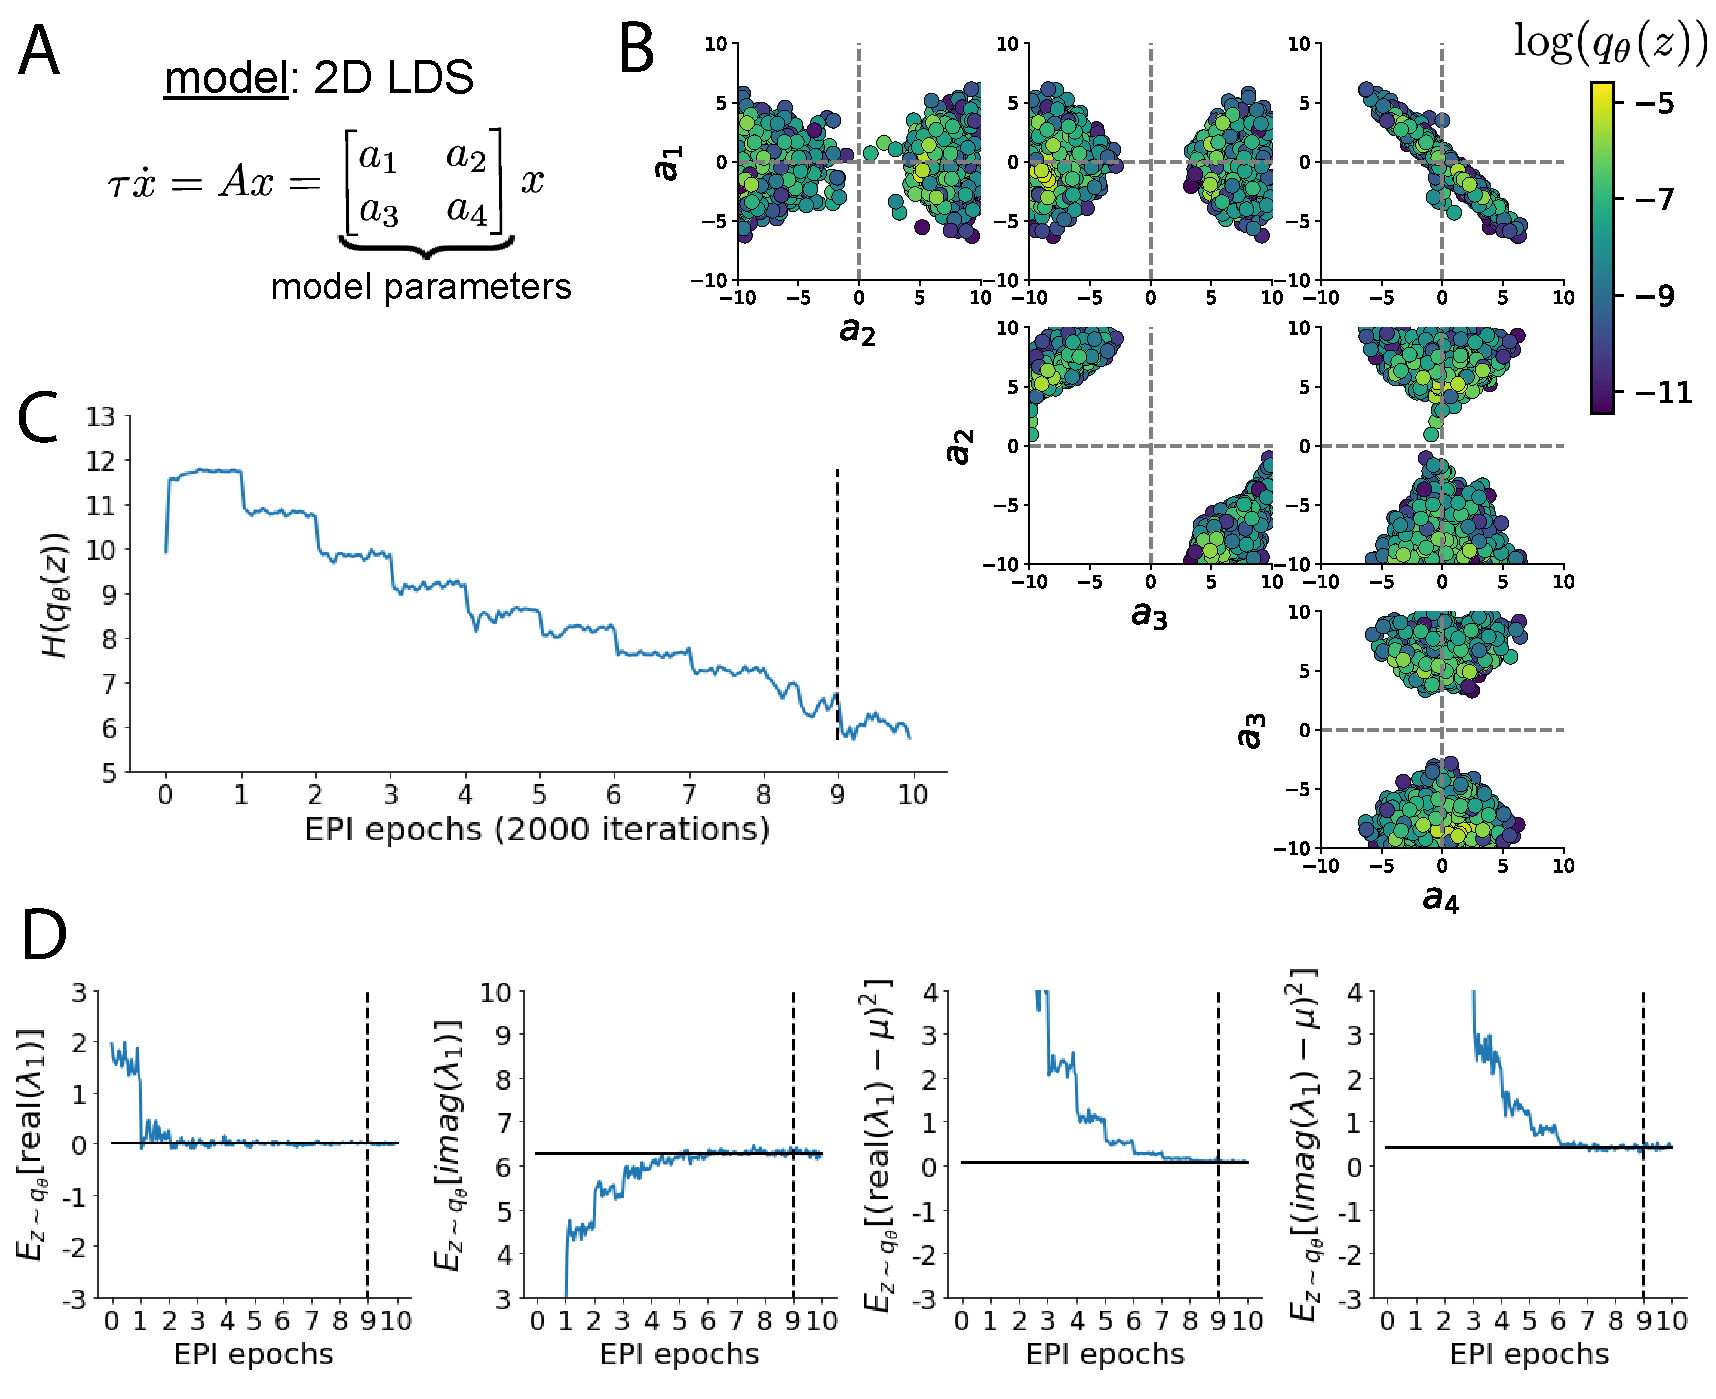
\includegraphics[scale=0.5]{figures/figS1/figS1.pdf}
\end{center}
Fig. S1: A. EPI for rank-1 networks doing discrimination. B. EPI for rank-2 networks doing context-dependent discrimination.
\end{figure}

\end{document}

